\chapter{Aurangabad et Hampi}
\section*{23 décembre 2015}
Une semaine pour revenir à Bangalore, j'en profite pour faire 2 étapes touristiques à Aurangabad et Hampi \newline
 Première partie : 22h de train entre Delhi et Aurangabad \newline
 \newline
\centerline{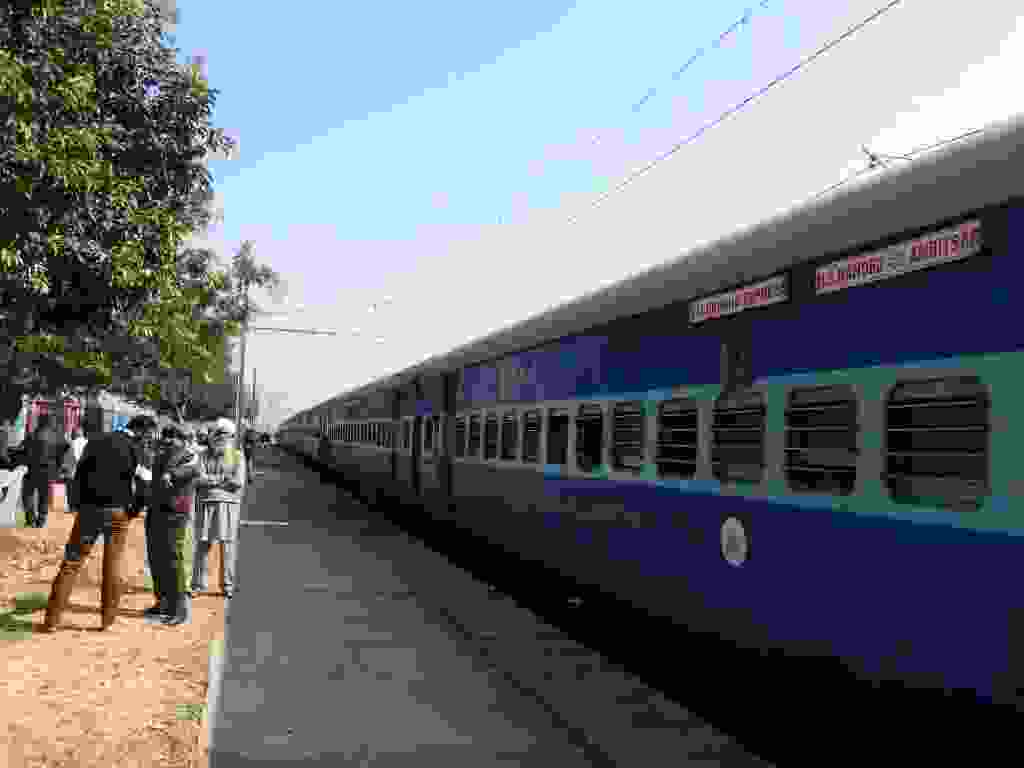
\includegraphics[width=\mywidth]{../wp-content/uploads/2015/12/wpid-oi000791-1024x768.jpg} } 
 \newline
 \newline
\centerline{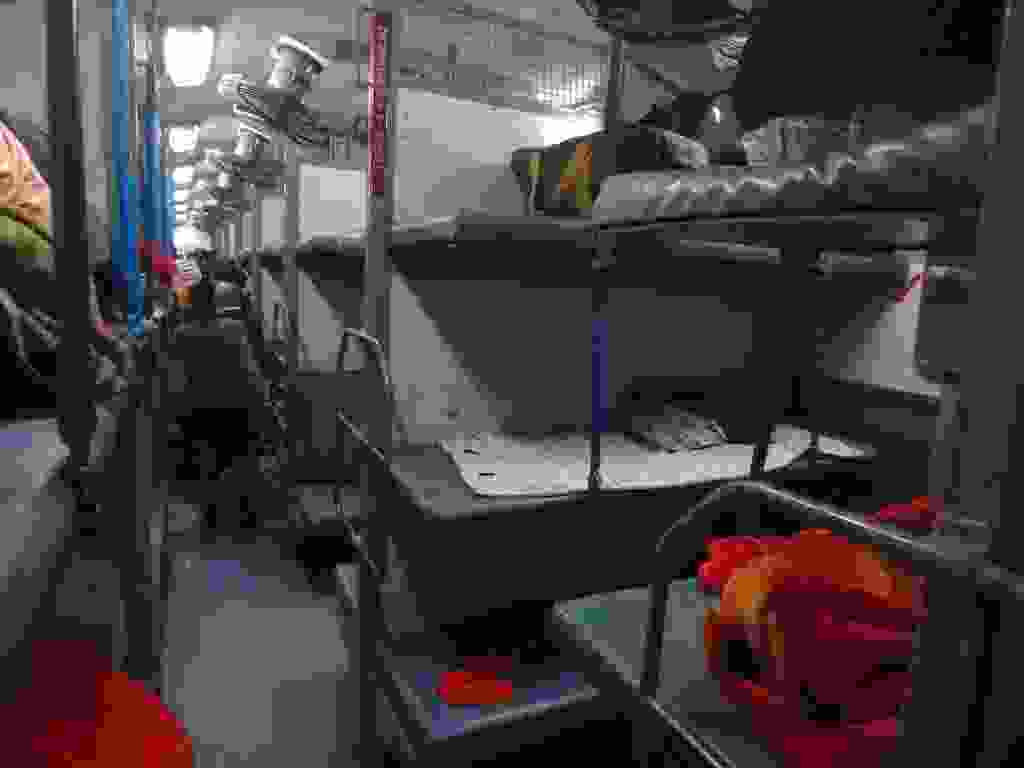
\includegraphics[width=\mywidth]{../wp-content/uploads/2015/12/wpid-oi000790-1024x768.jpg} } 
 \newline
 Une nuit dans un dortoir à l'indienne : 1.4€ \newline
 \newline
\centerline{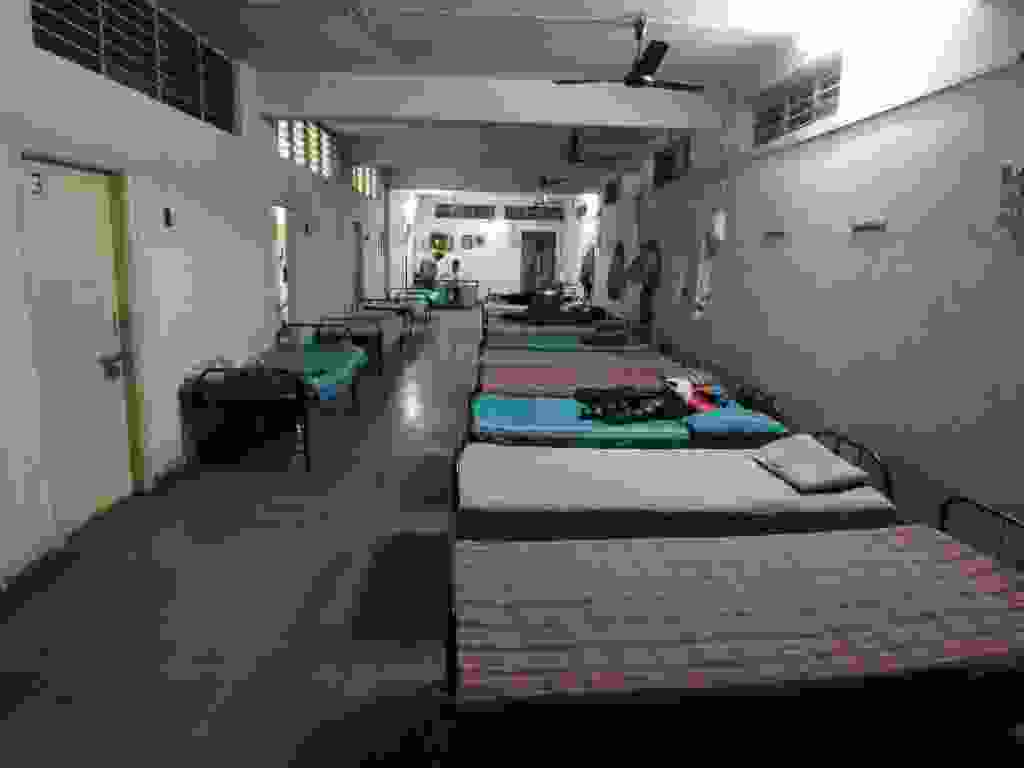
\includegraphics[width=\mywidth]{../wp-content/uploads/2015/12/wpid-oi000793-1024x768.jpg} } 
 \newline
 Ajanta à 90km d'Aurangabad : 30 grottes bouddhistes creusées dans la falaise entre le 2e siècle avant J-C et le 8e siècle \newline
 \newline
\centerline{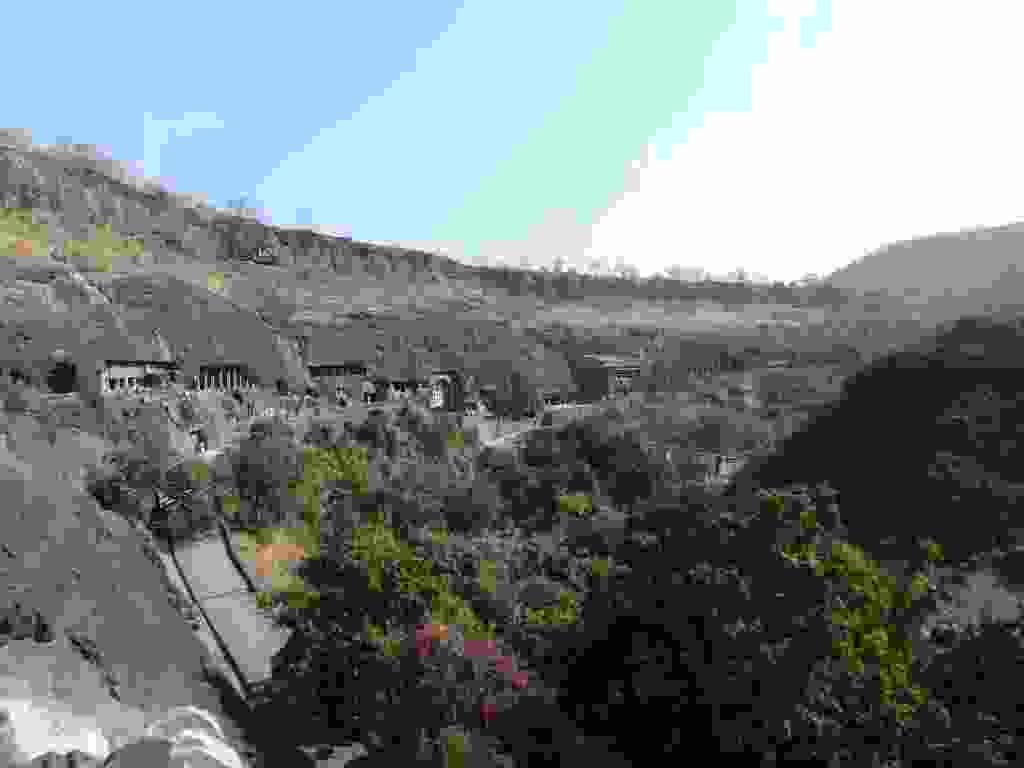
\includegraphics[width=\mywidth]{../wp-content/uploads/2015/12/PC151302-1024x768.jpg} } 
 \newline
 \newline
\centerline{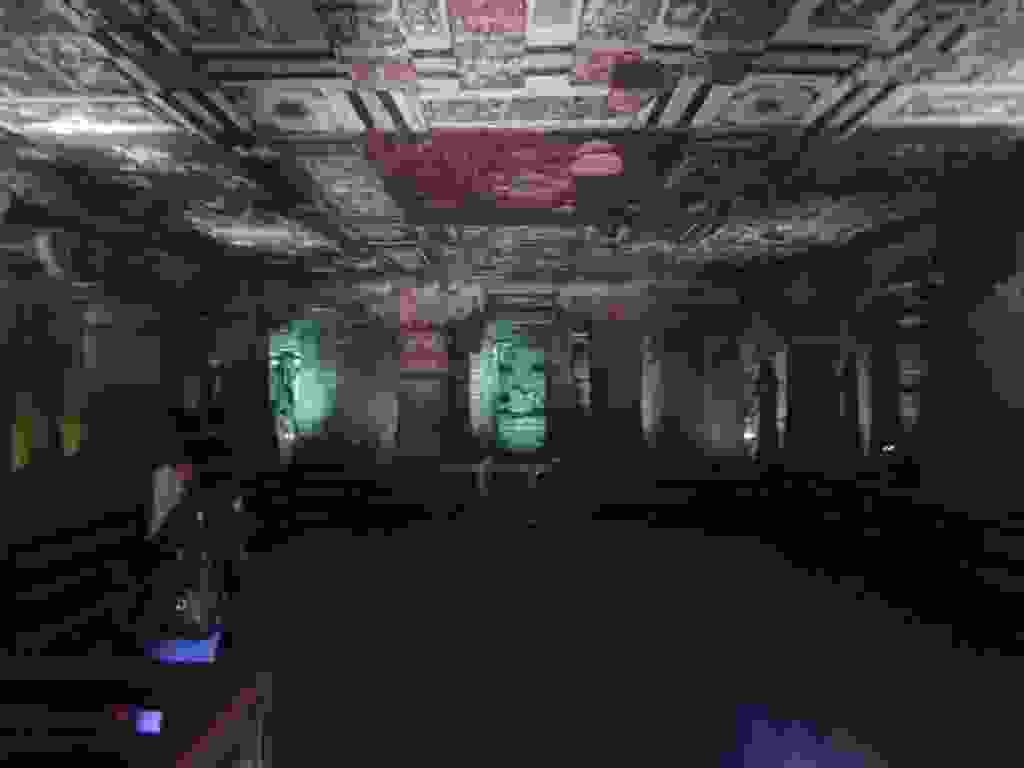
\includegraphics[width=\mywidth]{../wp-content/uploads/2015/12/PC151272-1024x768.jpg} } 
 \newline
 \newline
\centerline{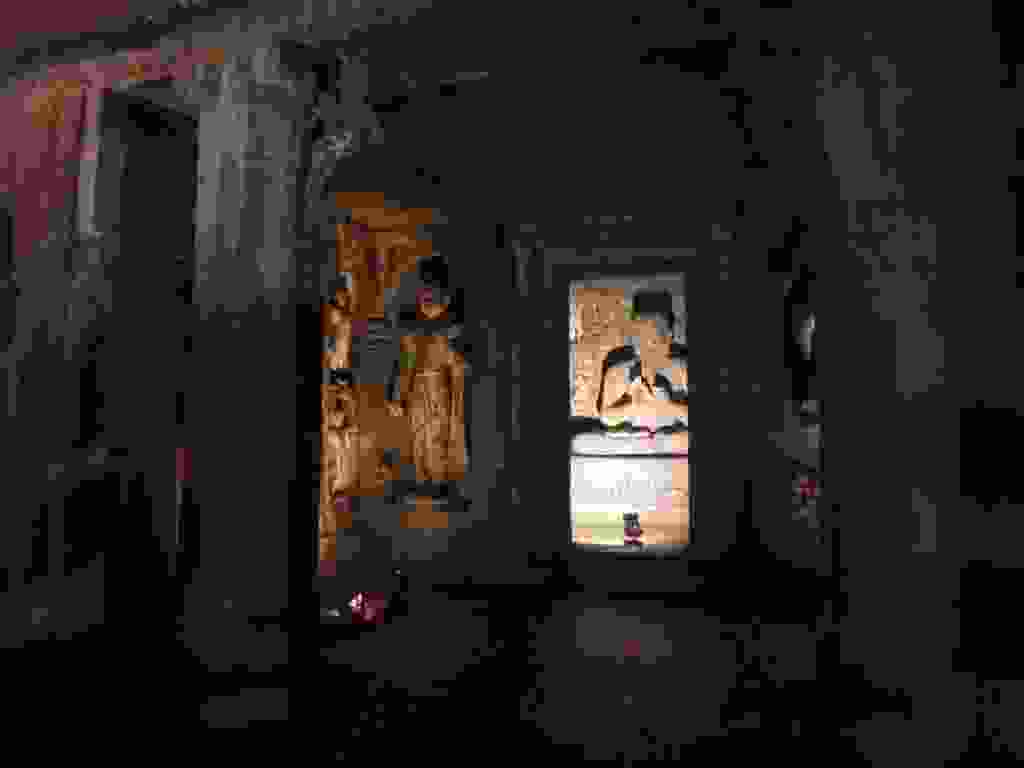
\includegraphics[width=\mywidth]{../wp-content/uploads/2015/12/PC151278-1024x768.jpg} } 
 \newline
 \newline
\centerline{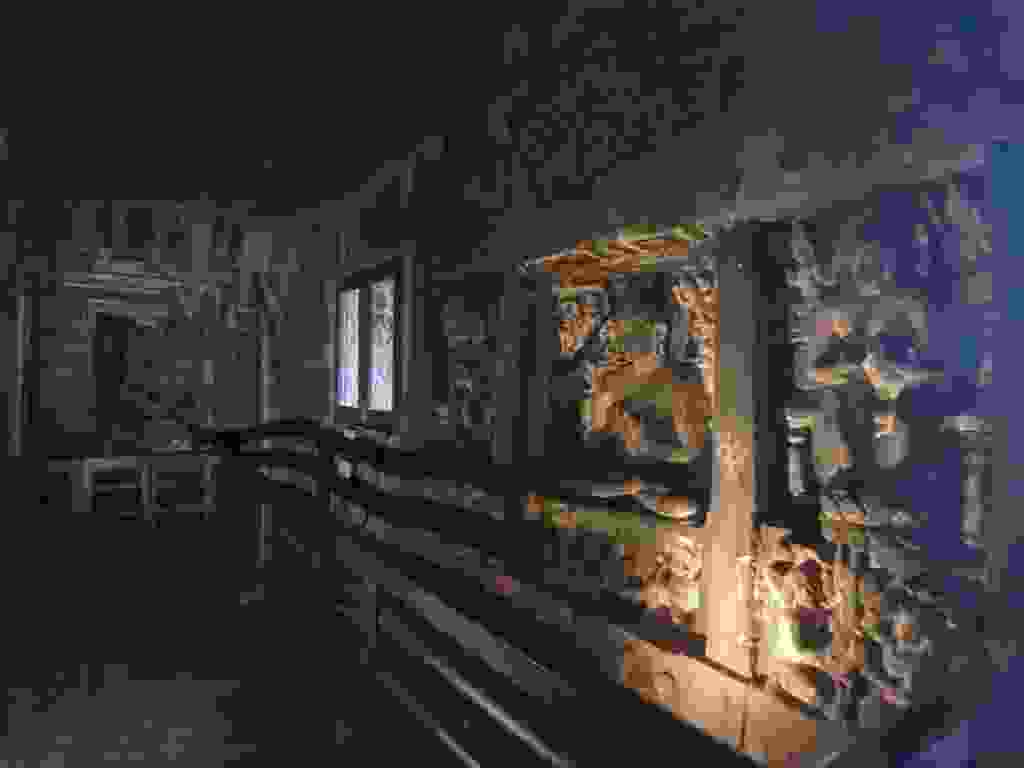
\includegraphics[width=\mywidth]{../wp-content/uploads/2015/12/PC151280-1024x768.jpg} } 
 \newline
 \newline
\centerline{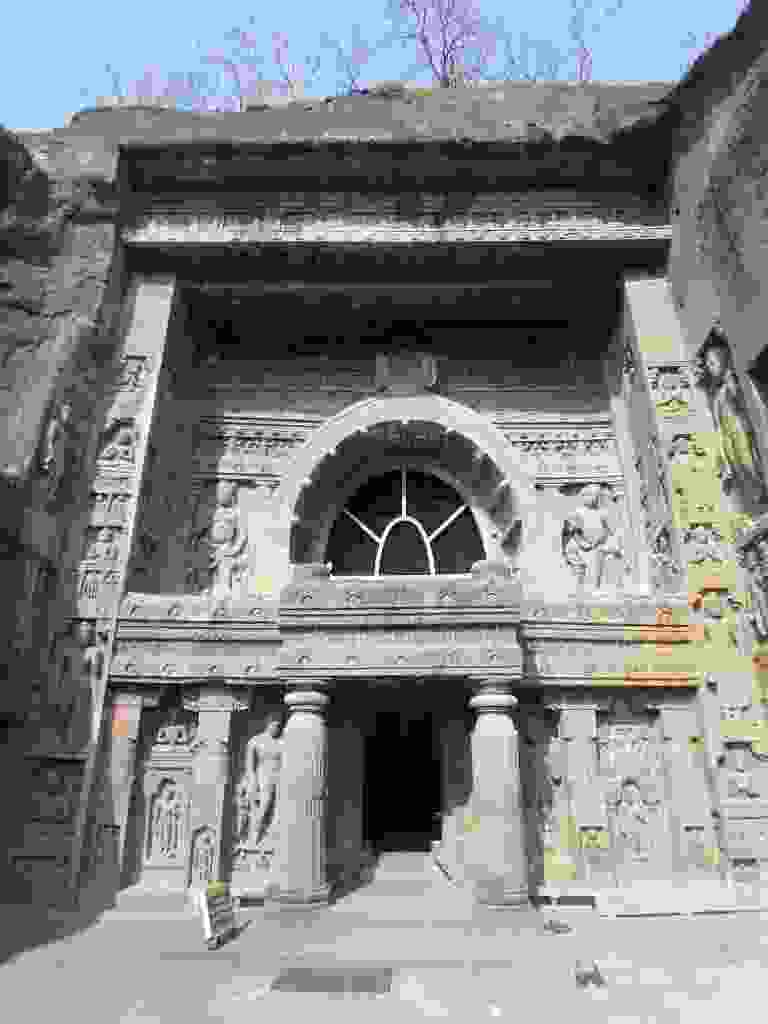
\includegraphics[width=\mywidth]{../wp-content/uploads/2015/12/PC151297-768x1024.jpg} } 
 \newline
 \newline
\centerline{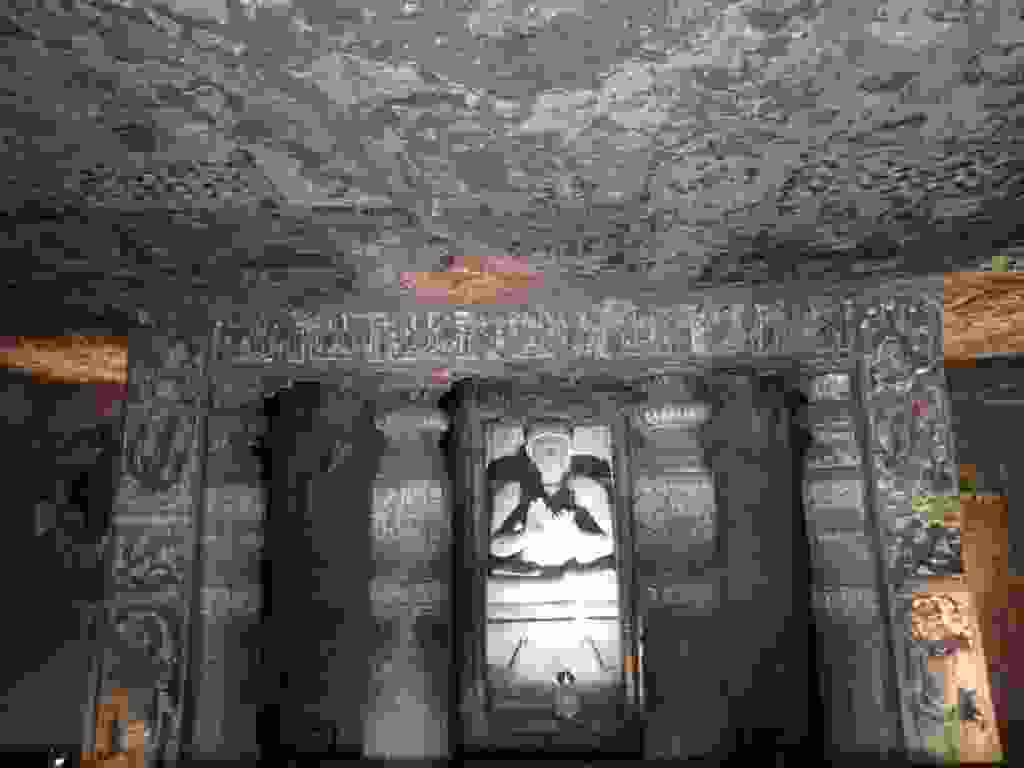
\includegraphics[width=\mywidth]{../wp-content/uploads/2015/12/PC151301-1024x768.jpg} } 
 \newline
 \newline
\centerline{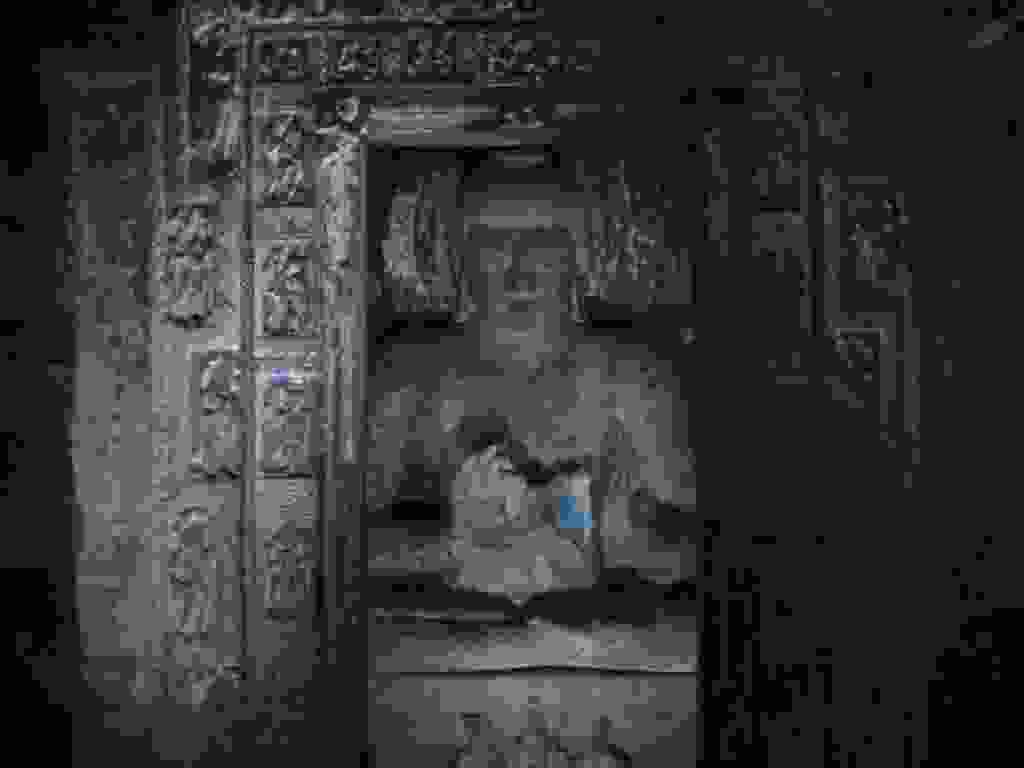
\includegraphics[width=\mywidth]{../wp-content/uploads/2015/12/PC151268-1024x768.jpg} } 
 \newline
 \newline
\centerline{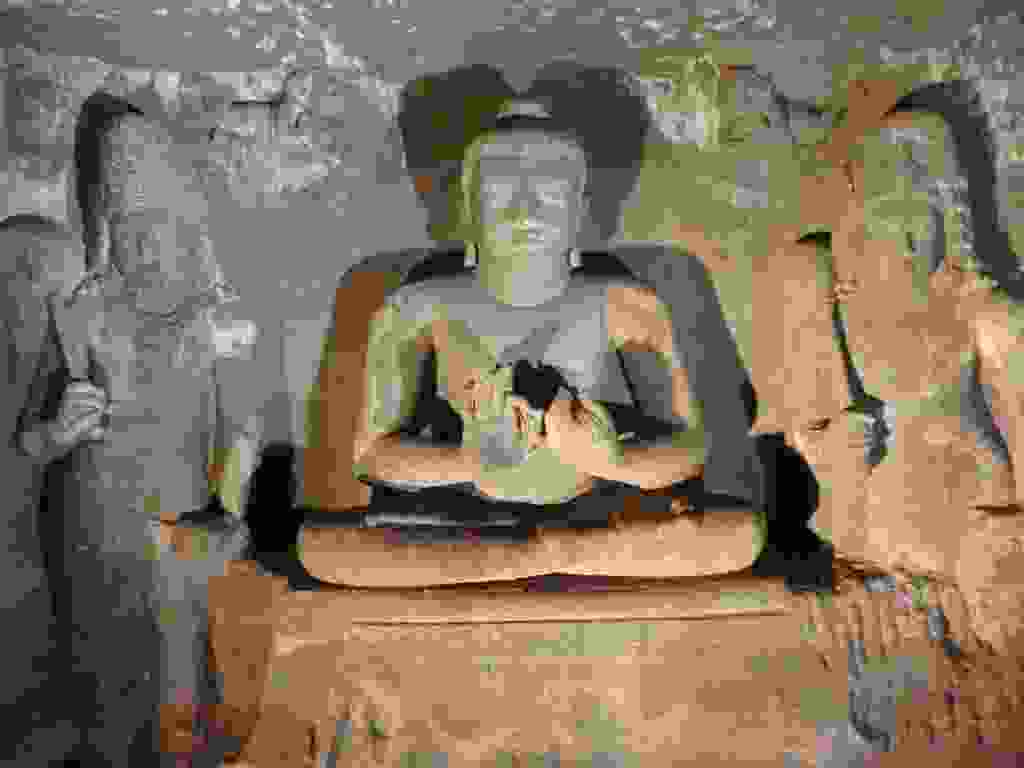
\includegraphics[width=\mywidth]{../wp-content/uploads/2015/12/PC151307-1024x768.jpg} } 
 \newline
 \newline
\centerline{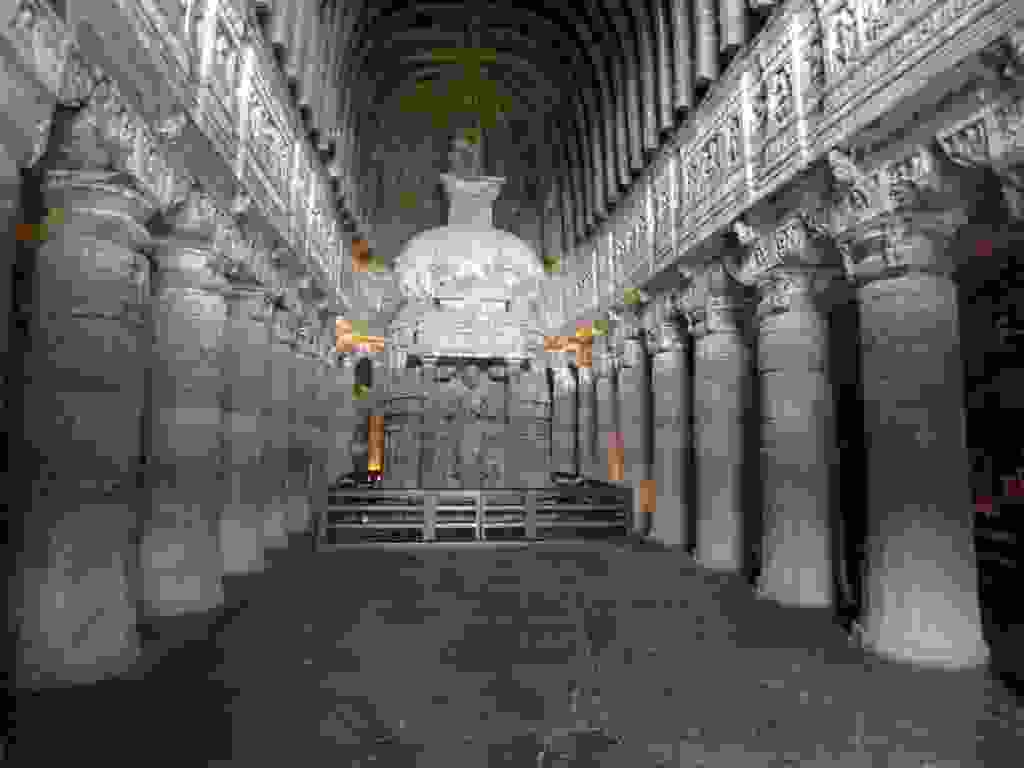
\includegraphics[width=\mywidth]{../wp-content/uploads/2015/12/PC151320-1024x768.jpg} } 
 \newline
 \newline
\centerline{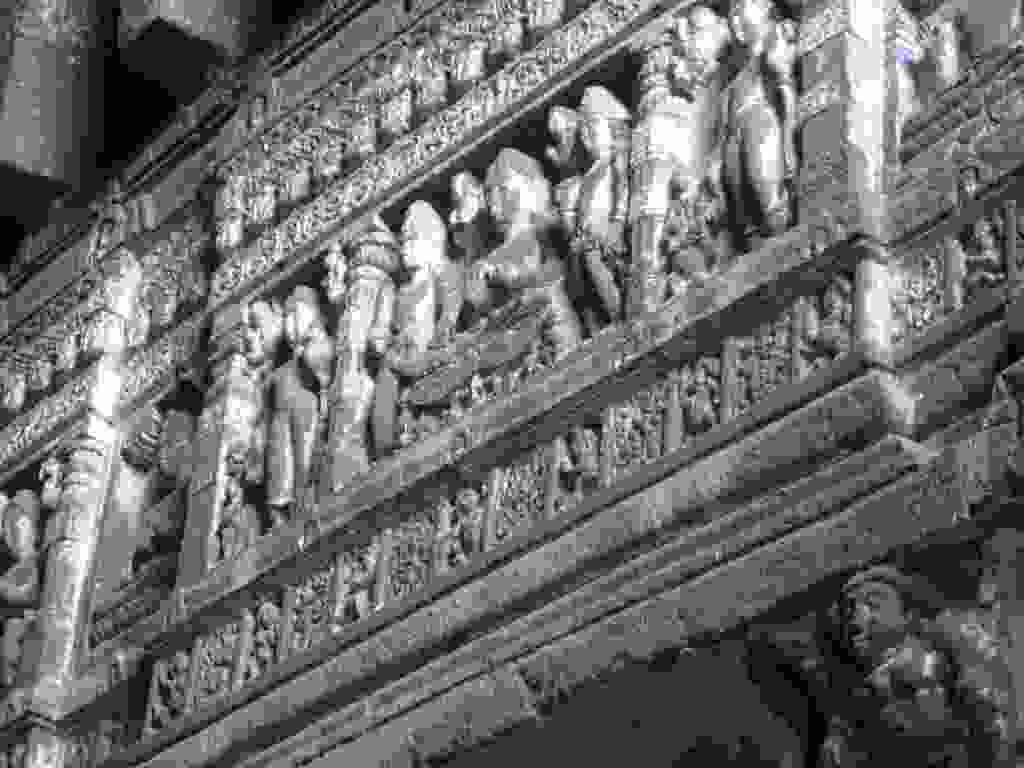
\includegraphics[width=\mywidth]{../wp-content/uploads/2015/12/PC151321-1024x768.jpg} } 
 \newline
 Restes de peintures \newline
 \newline
\centerline{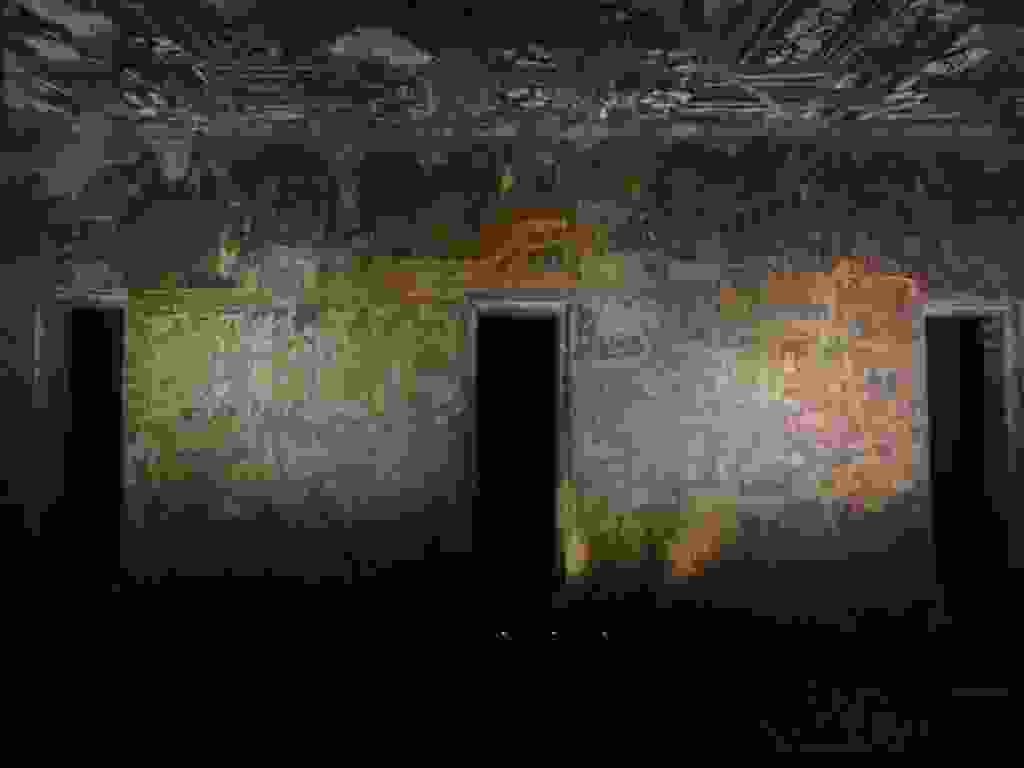
\includegraphics[width=\mywidth]{../wp-content/uploads/2015/12/PC151269-1024x768.jpg} } 
 \newline
 Beau site naturel autour des grottes, il doit y avoir de belles cascades pendant la saison des pluies \newline
 \newline
\centerline{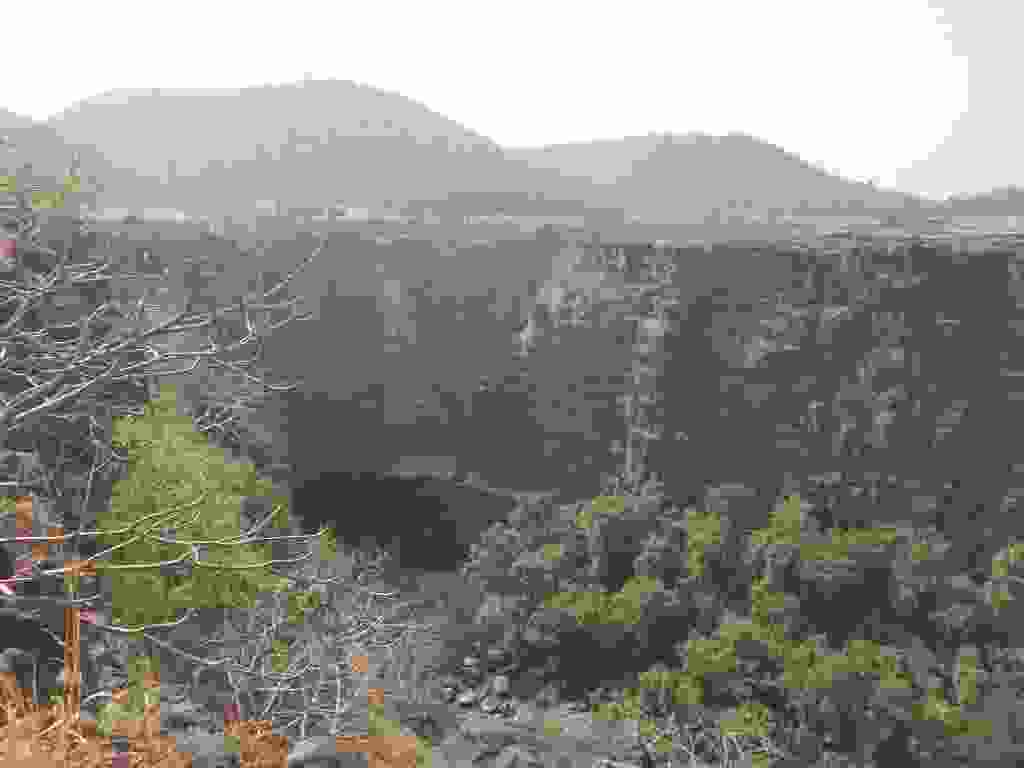
\includegraphics[width=\mywidth]{../wp-content/uploads/2015/12/PC151325-1024x768.jpg} } 
 \newline
 Je rencontre un indien qui me fait visiter son village juste au dessus d'Ajanta : très tranquille, pas de voiture donc pas de klaxons incessants comme partout ailleurs \newline
 \newline
\centerline{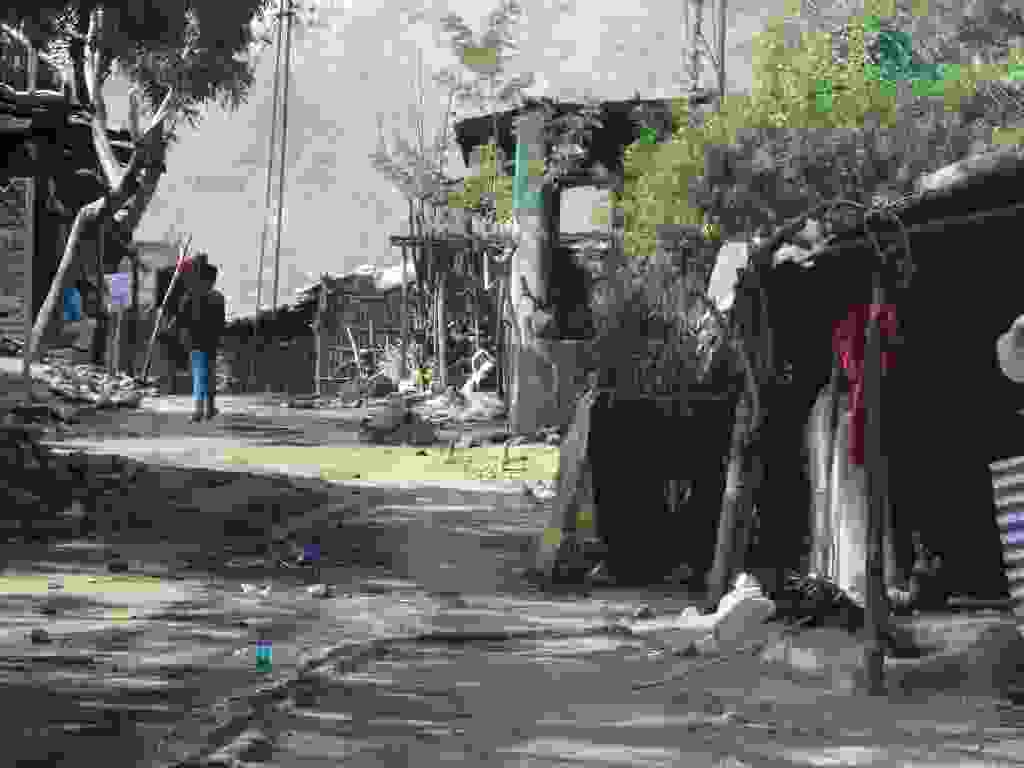
\includegraphics[width=\mywidth]{../wp-content/uploads/2015/12/PC151327-1024x768.jpg} } 
 \newline
 \newline
\centerline{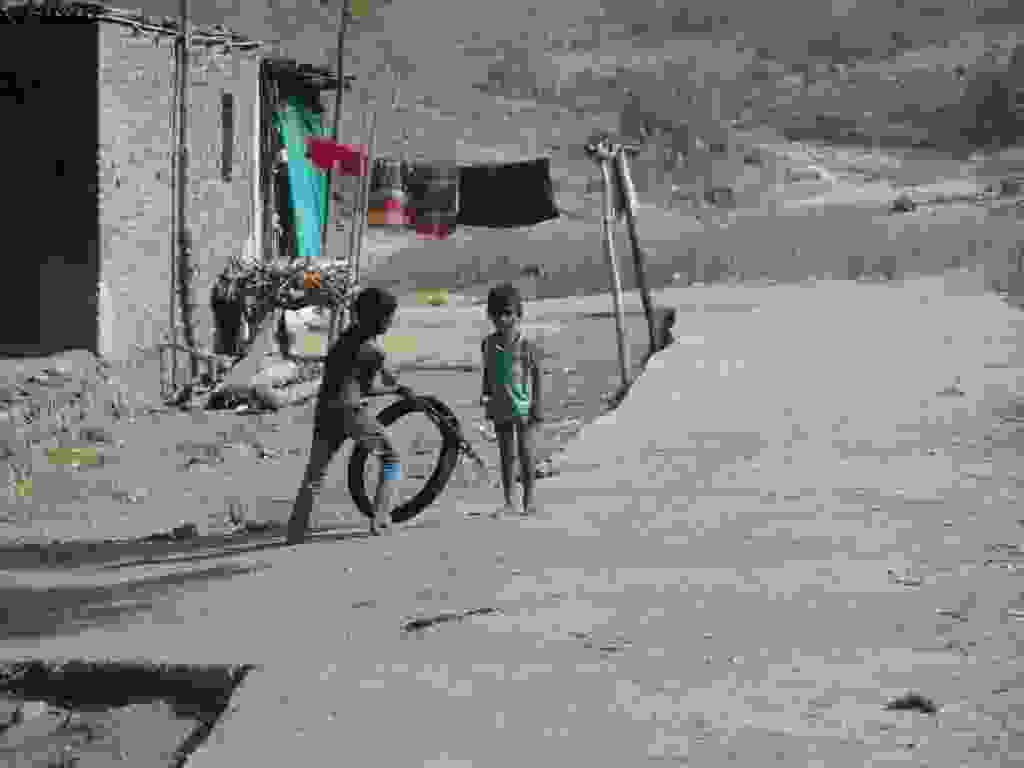
\includegraphics[width=\mywidth]{../wp-content/uploads/2015/12/PC151328-1024x768.jpg} } 
 \newline
 \newline
\centerline{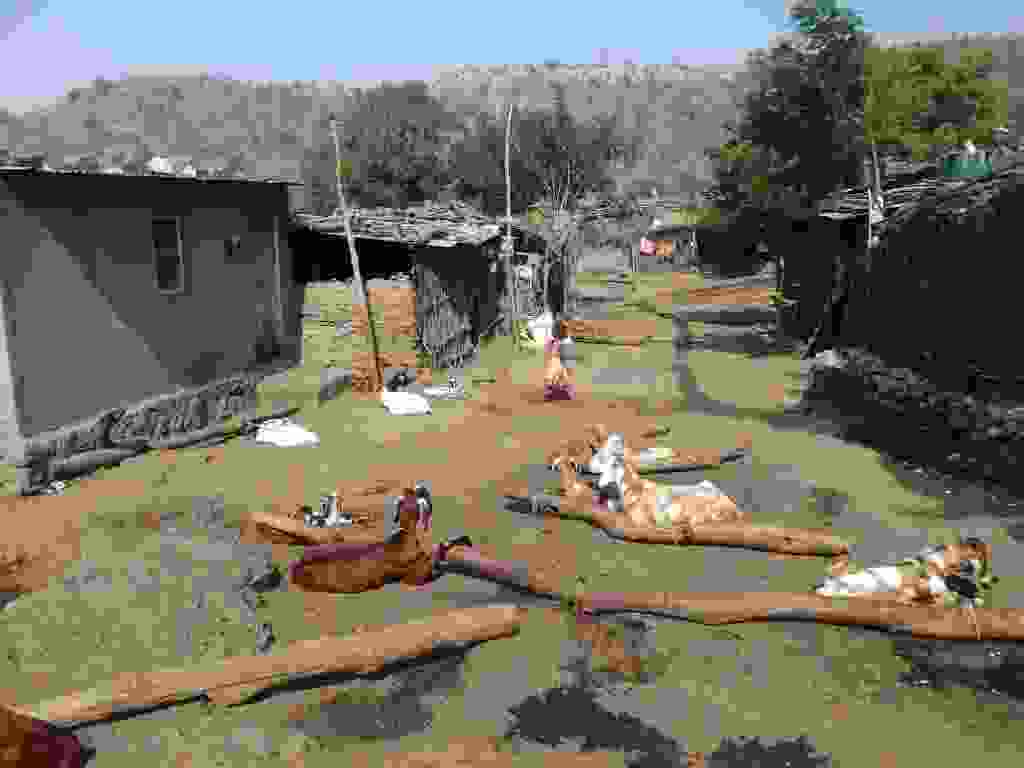
\includegraphics[width=\mywidth]{../wp-content/uploads/2015/12/PC151329-1024x768.jpg} } 
 \newline
 L'école du village \newline
 \newline
\centerline{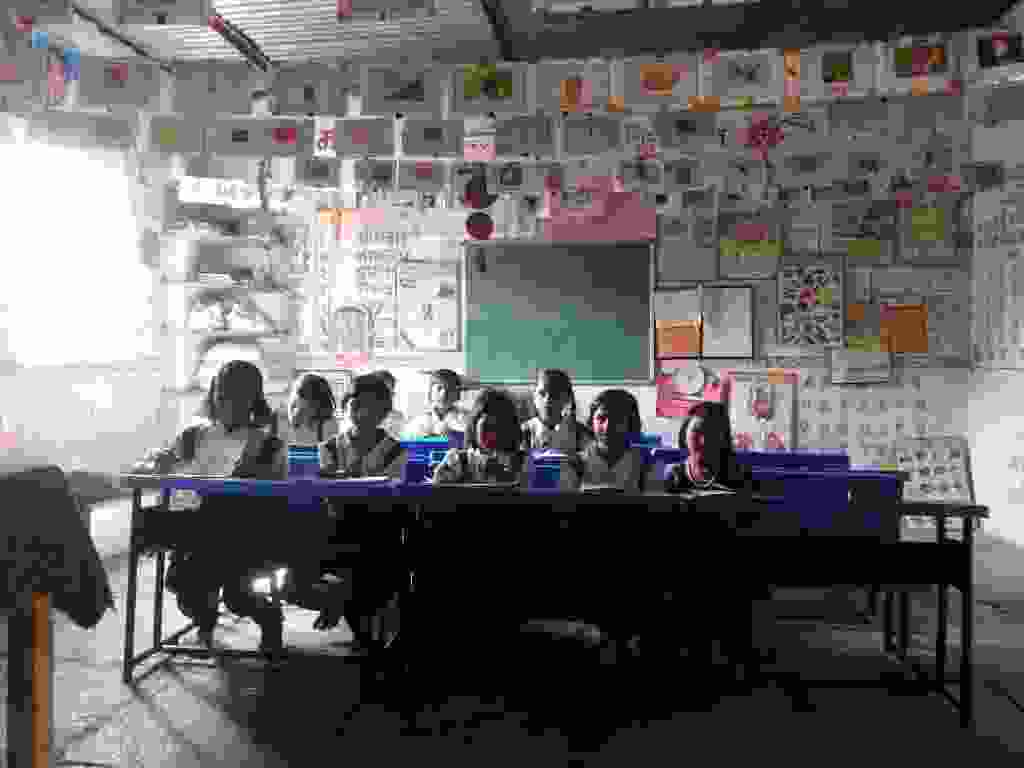
\includegraphics[width=\mywidth]{../wp-content/uploads/2015/12/PC151330-1024x768.jpg} } 
 \newline
 Ellora juste à côté d'Aurangabad : un mélange de grottes hindoues, jainistes et bouddhistes \newline
 Temple hindou de Kailasanatha, entièrement excavé dans la falaise \newline
 \newline
\centerline{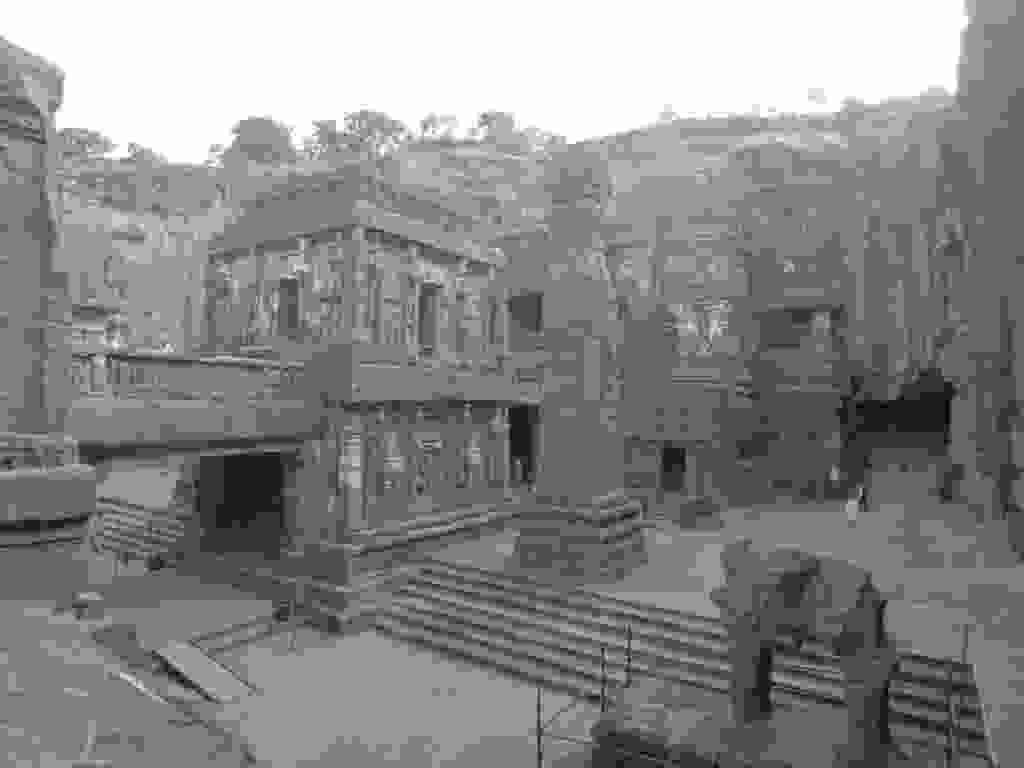
\includegraphics[width=\mywidth]{../wp-content/uploads/2015/12/PC161360-1024x768.jpg} } 
 \newline
 \newline
\centerline{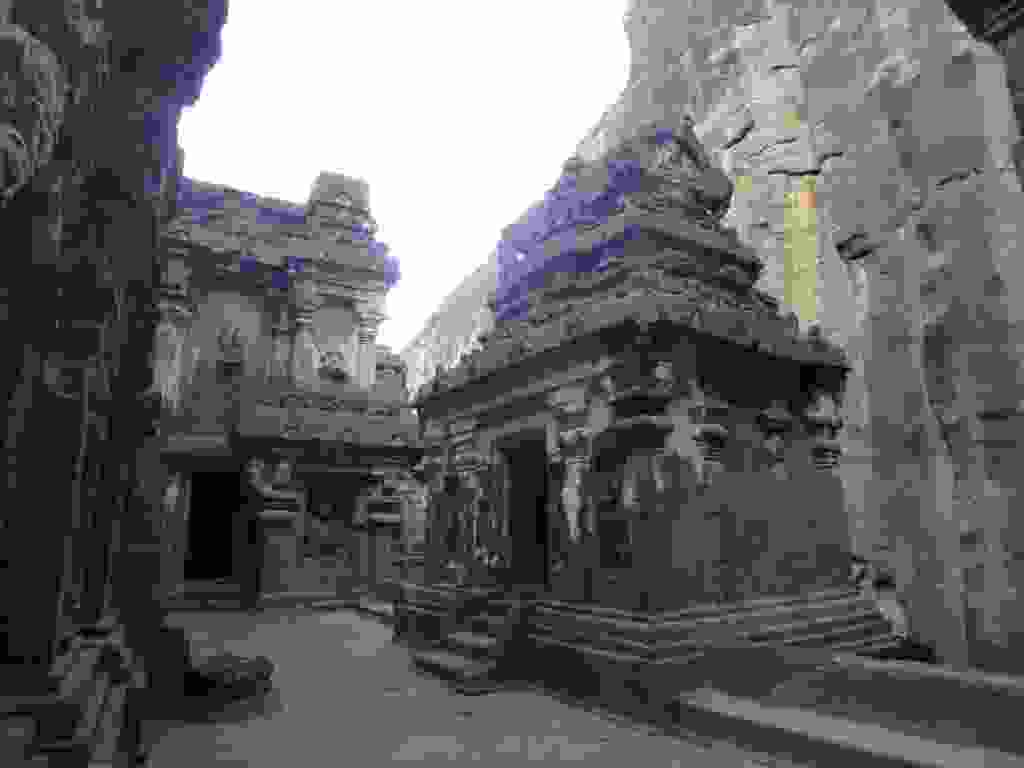
\includegraphics[width=\mywidth]{../wp-content/uploads/2015/12/PC161356-1024x768.jpg} } 
 \newline
 Groupe de 4 grottes jainistes \newline
 \newline
\centerline{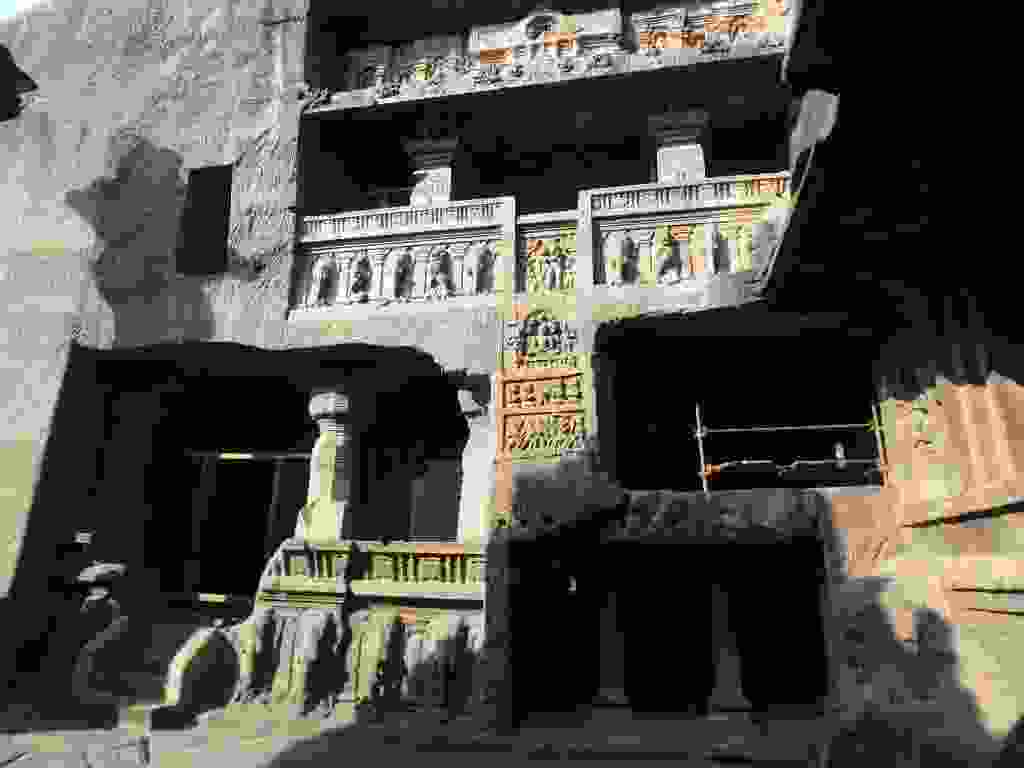
\includegraphics[width=\mywidth]{../wp-content/uploads/2015/12/PC161387-1024x768.jpg} } 
 \newline
 \newline
\centerline{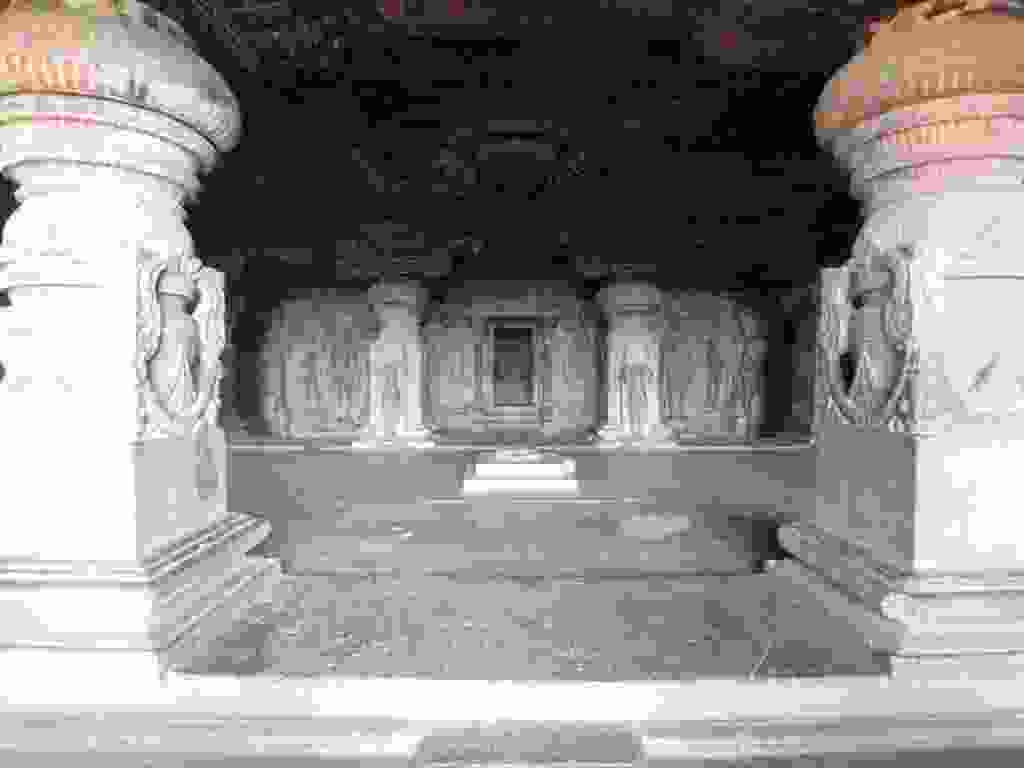
\includegraphics[width=\mywidth]{../wp-content/uploads/2015/12/PC161390-1024x768.jpg} } 
 \newline
 \newline
\centerline{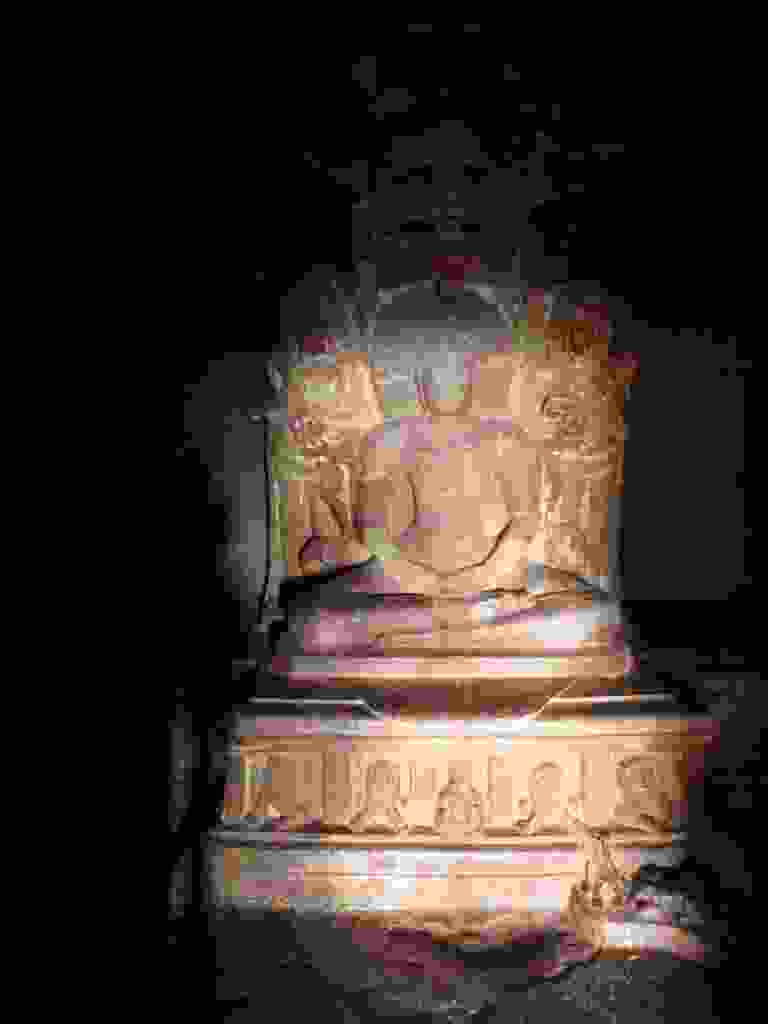
\includegraphics[width=\mywidth]{../wp-content/uploads/2015/12/PC161392-768x1024.jpg} } 
 \newline
 Une dizaines de grottes bouddhistes, ayant servies de temple ou de monastère, ça attire des touristes particuliers \newline
 \newline
\centerline{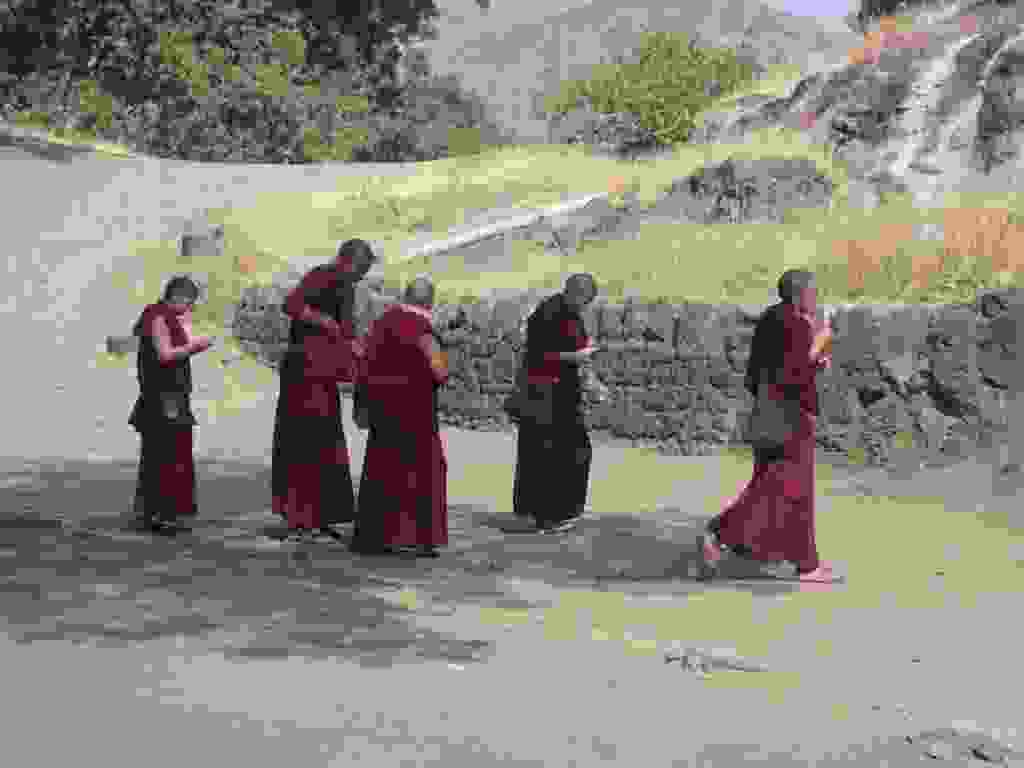
\includegraphics[width=\mywidth]{../wp-content/uploads/2015/12/PC161409-1024x768.jpg} } 
 \newline
 \newline
\centerline{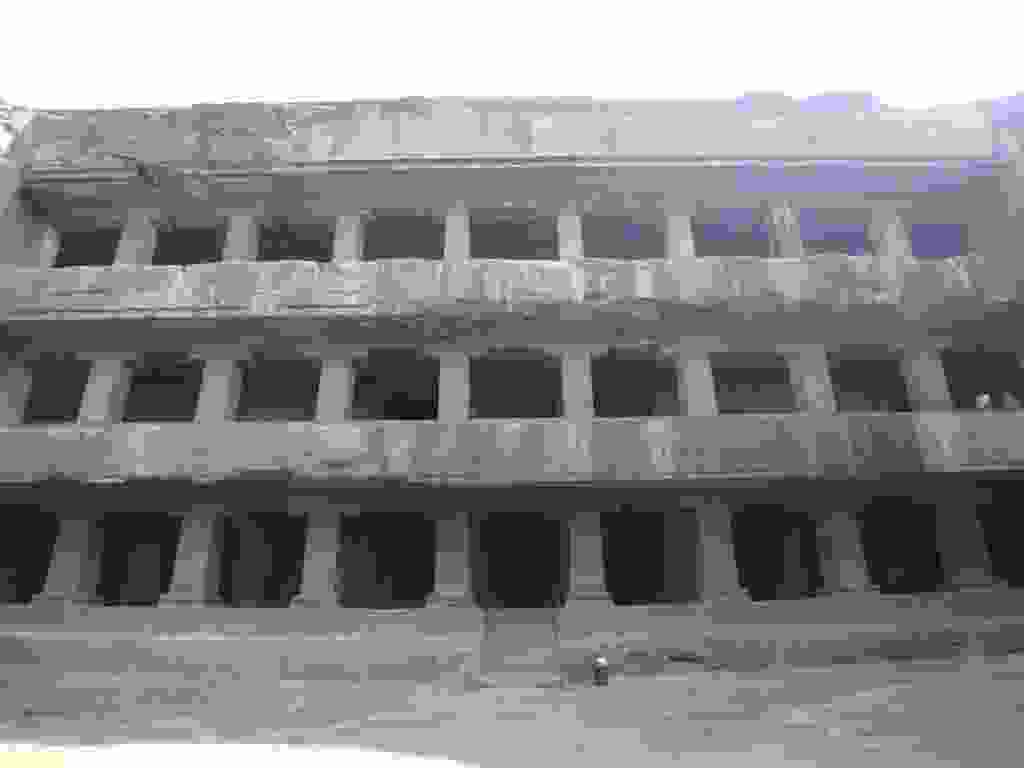
\includegraphics[width=\mywidth]{../wp-content/uploads/2015/12/PC161410-1024x768.jpg} } 
 \newline
 \newline
\centerline{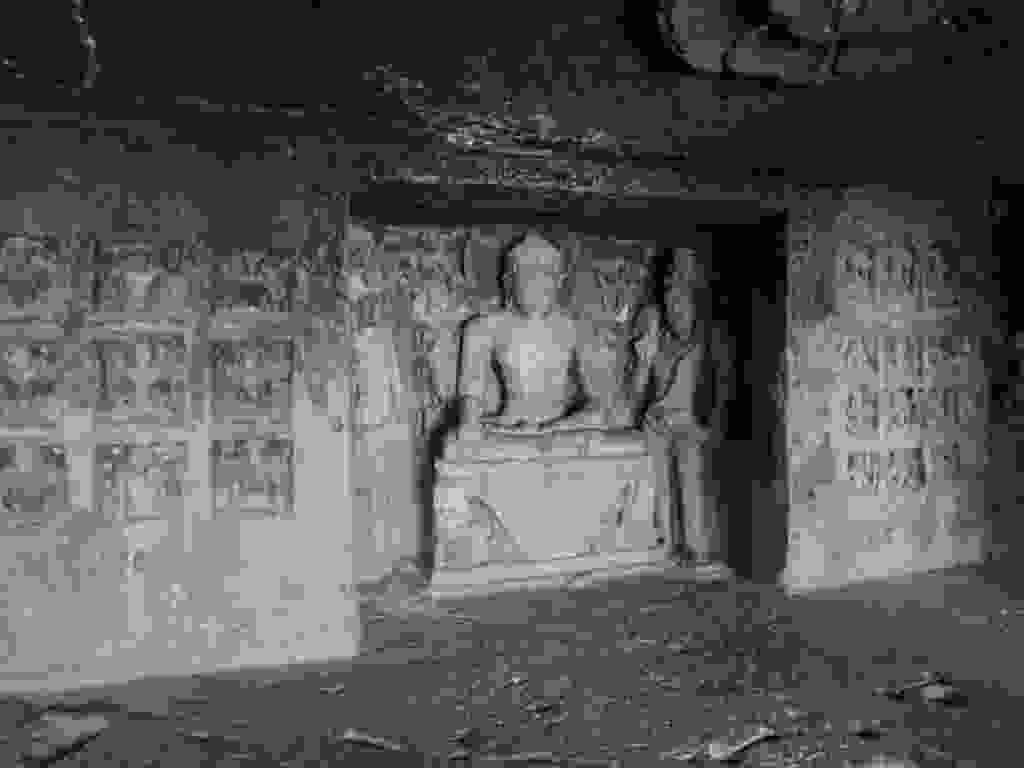
\includegraphics[width=\mywidth]{../wp-content/uploads/2015/12/PC161411-1024x768.jpg} } 
 \newline
 \newline
\centerline{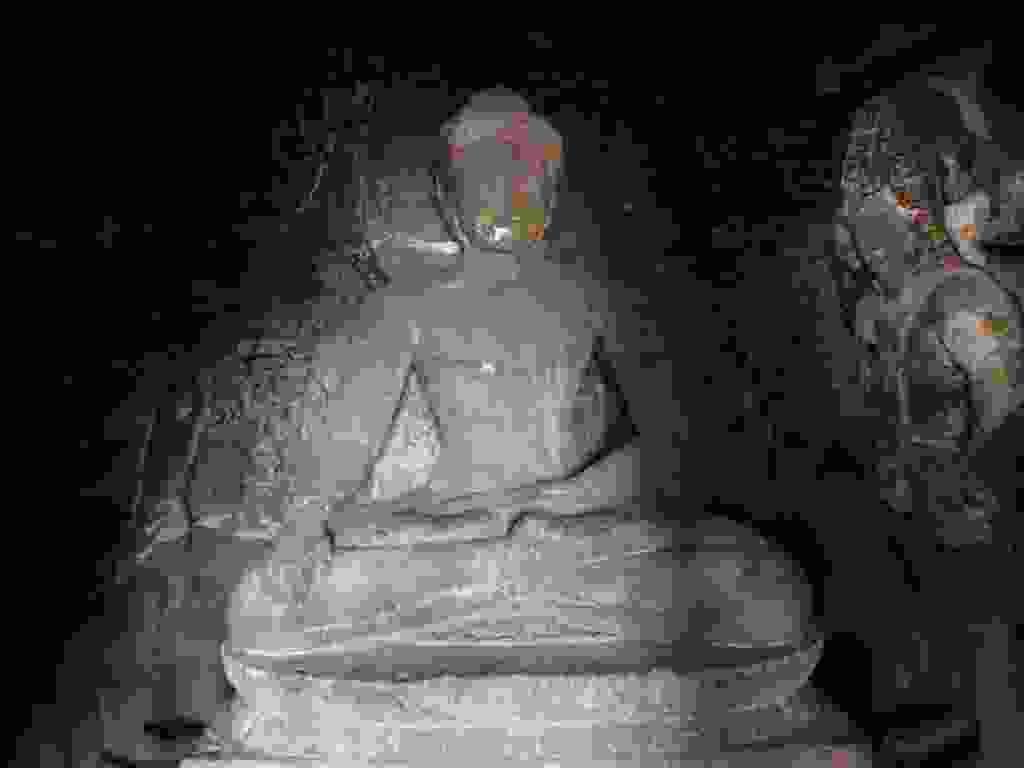
\includegraphics[width=\mywidth]{../wp-content/uploads/2015/12/PC161416-1024x768.jpg} } 
 \newline
 \newline
\centerline{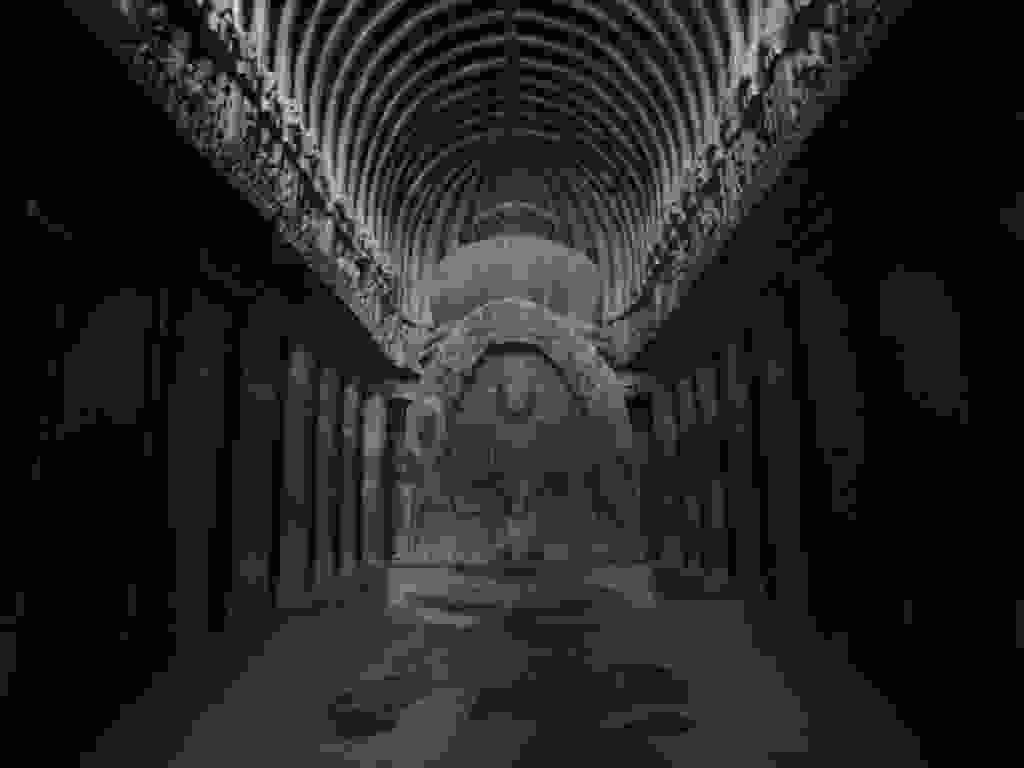
\includegraphics[width=\mywidth]{../wp-content/uploads/2015/12/PC161418-1024x768.jpg} } 
 \newline
 \newline
\centerline{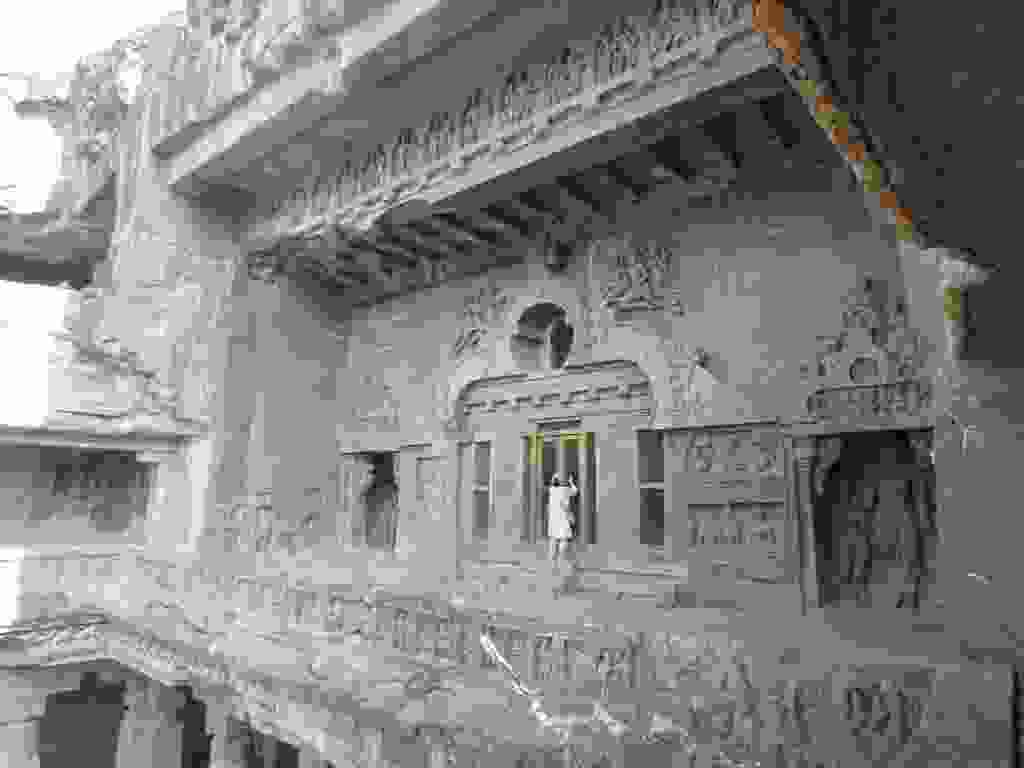
\includegraphics[width=\mywidth]{../wp-content/uploads/2015/12/PC161420-1024x768.jpg} } 
 \newline
 \newline
\centerline{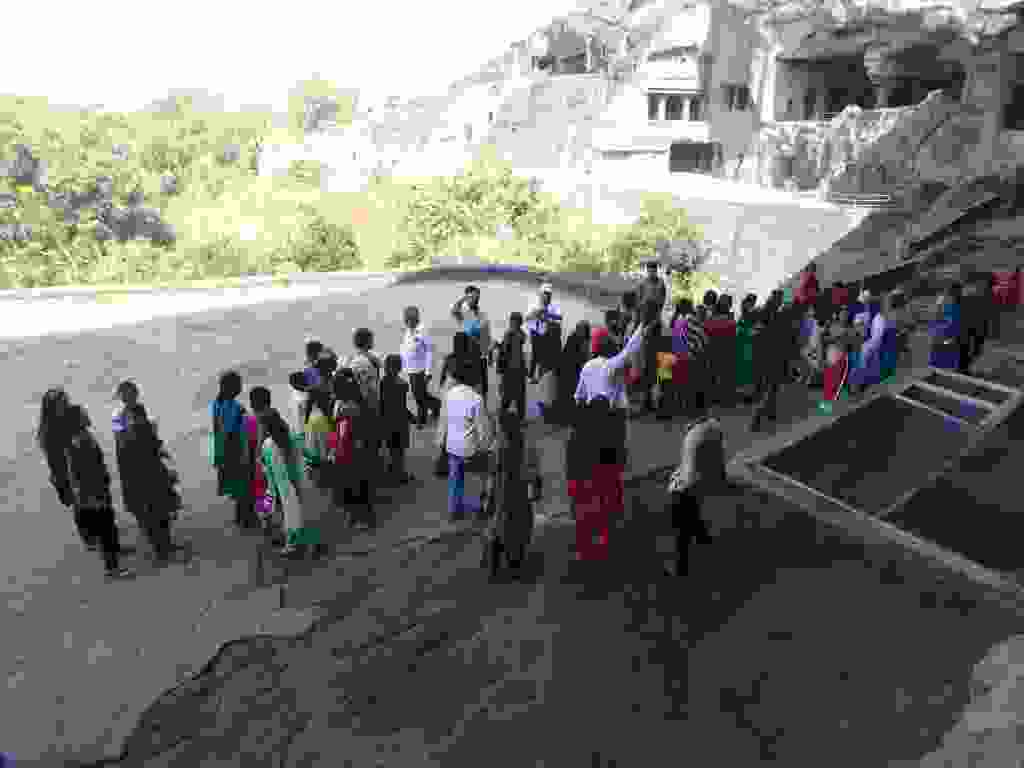
\includegraphics[width=\mywidth]{../wp-content/uploads/2015/12/PC161428-1024x768.jpg} } 
 \newline
 Je prends ensuite le bus pour rejoindre le village d'Hampi, il m'avait été conseillé par plusieurs voyageurs que j'ai rencontrés \newline
 \newline
\centerline{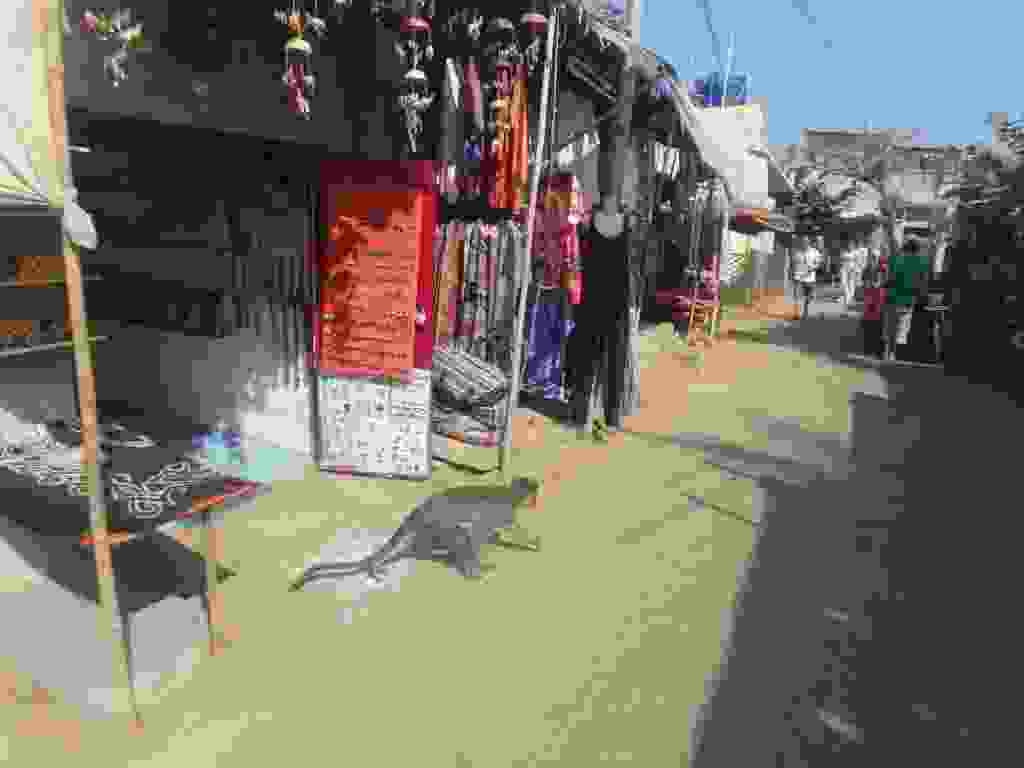
\includegraphics[width=\mywidth]{../wp-content/uploads/2015/12/PC181547-1024x768.jpg} } 
 \newline
 Cadre naturel très particulier : des cailloux partout \newline
 \newline
\centerline{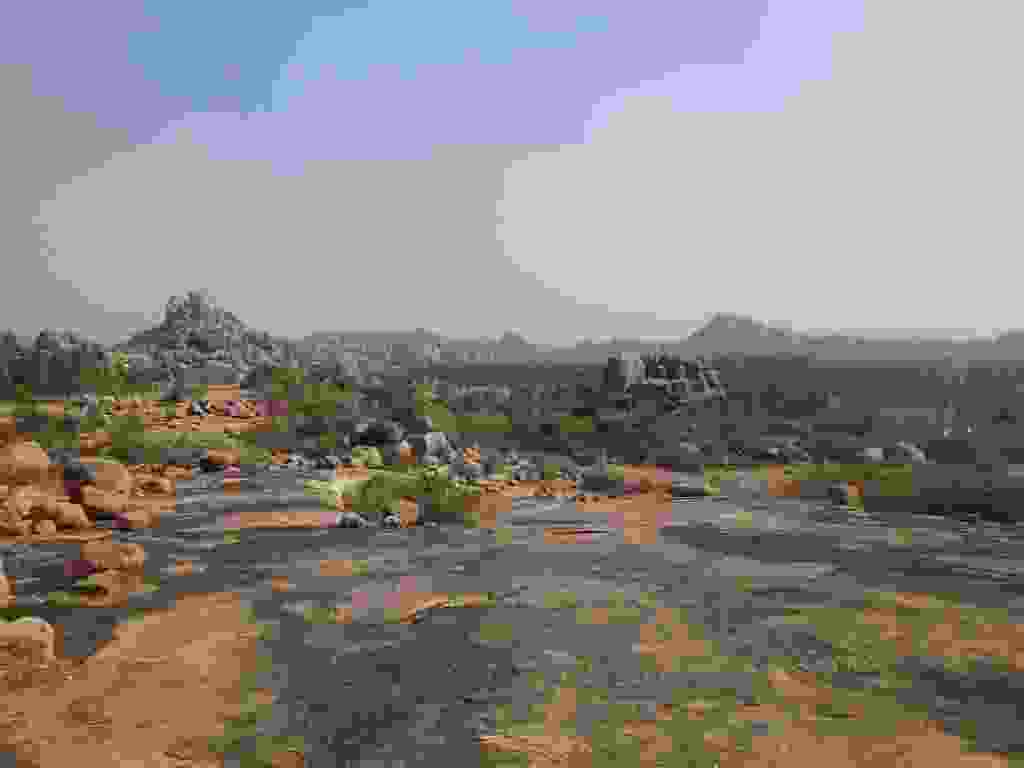
\includegraphics[width=\mywidth]{../wp-content/uploads/2015/12/PC171439-1024x768.jpg} } 
 \newline
 \newline
\centerline{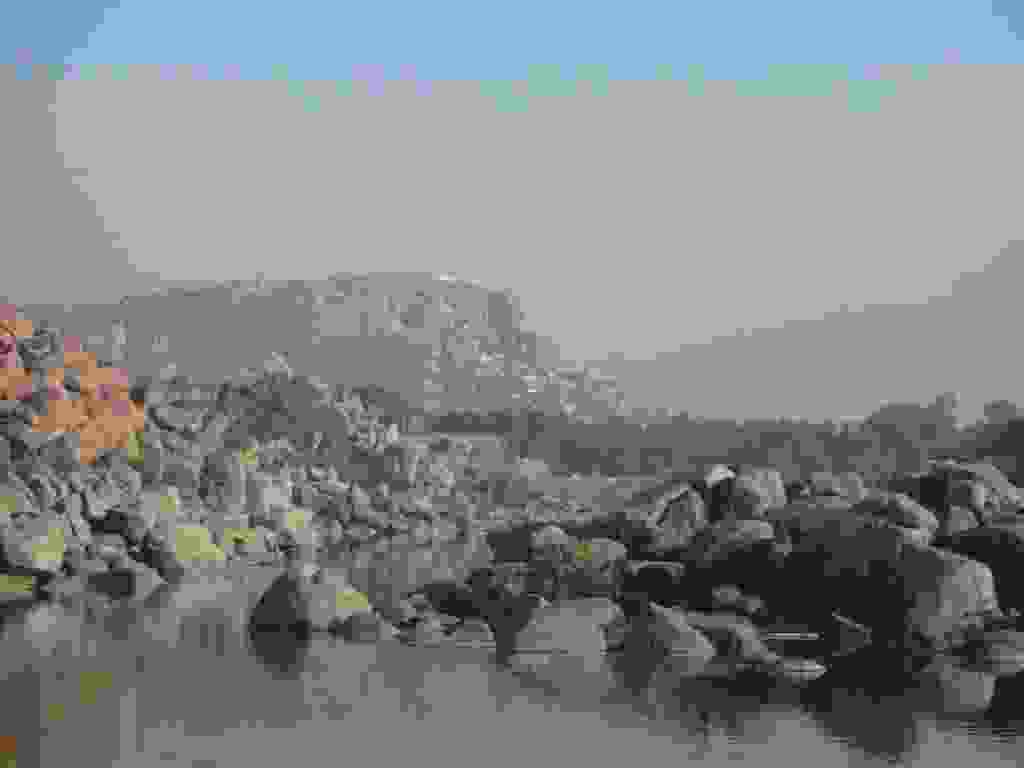
\includegraphics[width=\mywidth]{../wp-content/uploads/2015/12/PC181469-1024x768.jpg} } 
 \newline
 \newline
\centerline{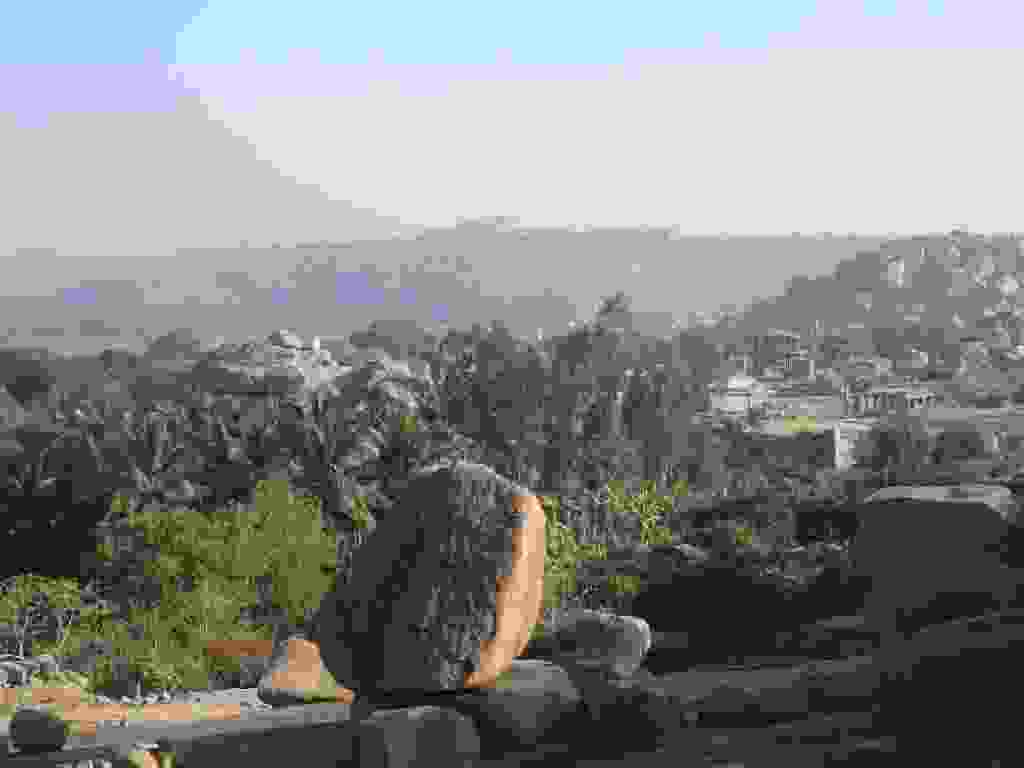
\includegraphics[width=\mywidth]{../wp-content/uploads/2015/12/PC181478-1024x768.jpg} } 
 \newline
 \newline
\centerline{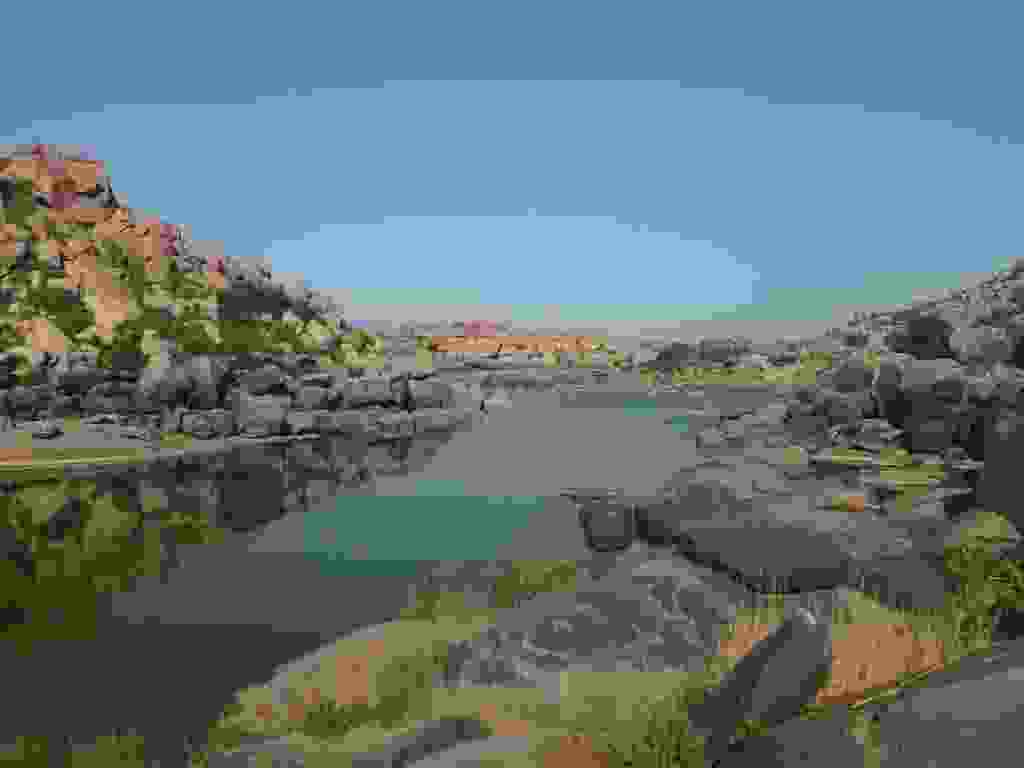
\includegraphics[width=\mywidth]{../wp-content/uploads/2015/12/PC181550-1024x768.jpg} } 
 \newline
 Monkey temple en haut d'une colline \newline
 \newline
\centerline{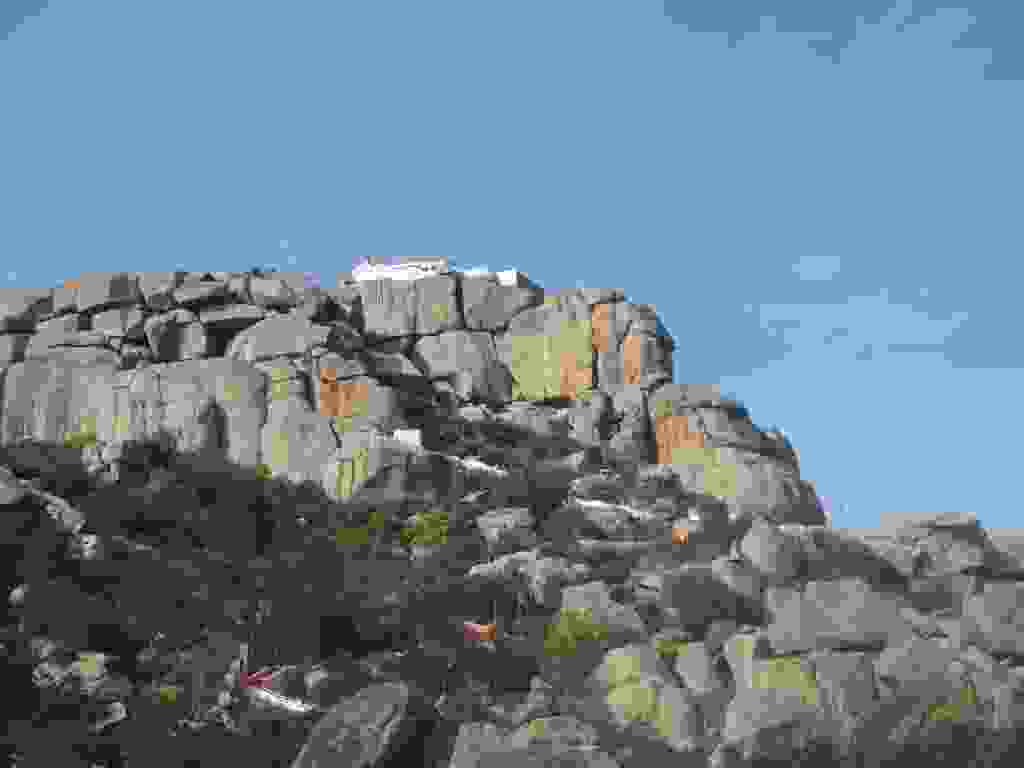
\includegraphics[width=\mywidth]{../wp-content/uploads/2015/12/PC171456-1024x768.jpg} } 
 \newline
 \newline
\centerline{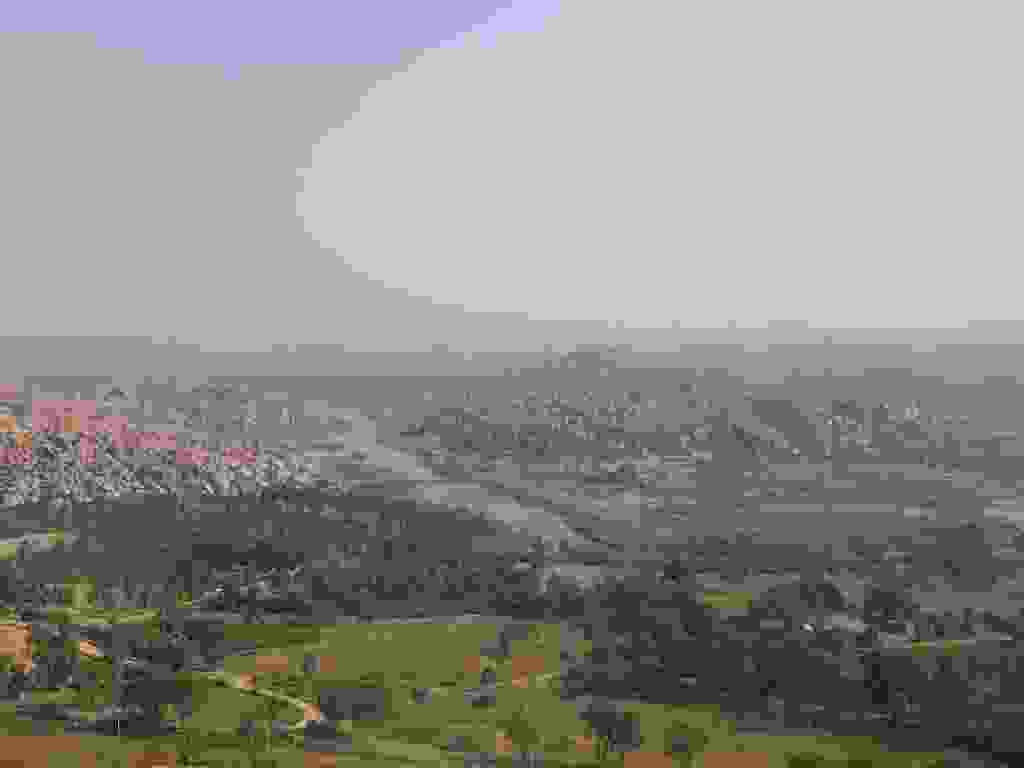
\includegraphics[width=\mywidth]{../wp-content/uploads/2015/12/PC171453-1024x768.jpg} } 
 \newline
 Temple principal Virupaksha \newline
 \newline
\centerline{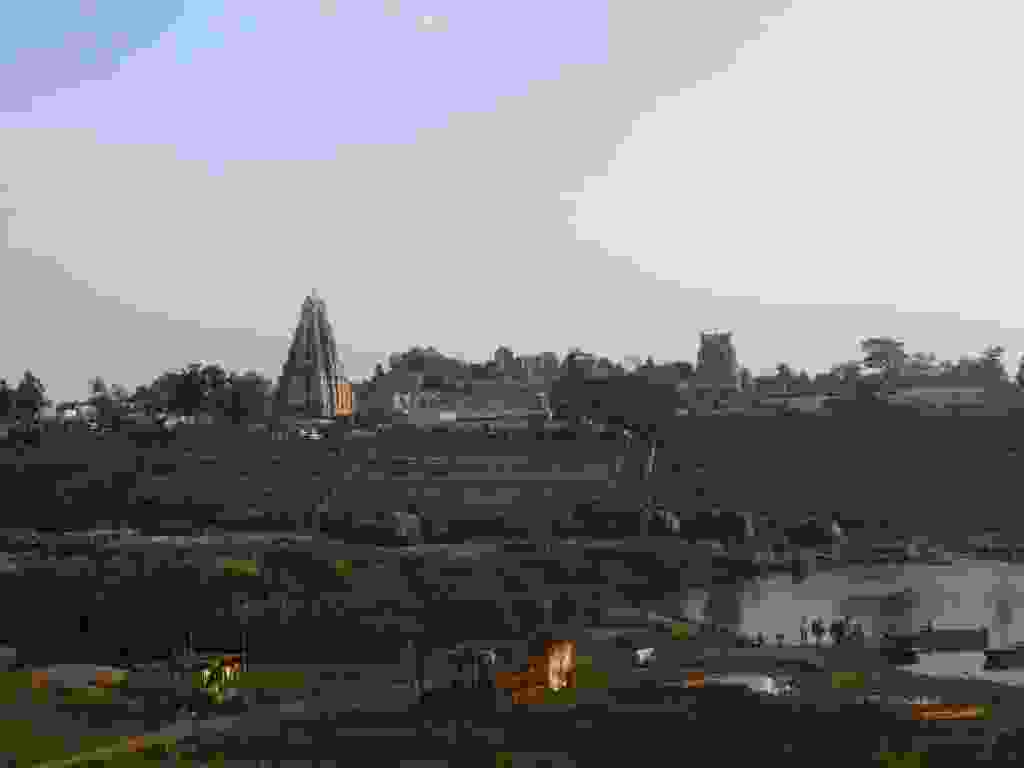
\includegraphics[width=\mywidth]{../wp-content/uploads/2015/12/PC171460-1024x768.jpg} } 
 \newline
 \newline
\centerline{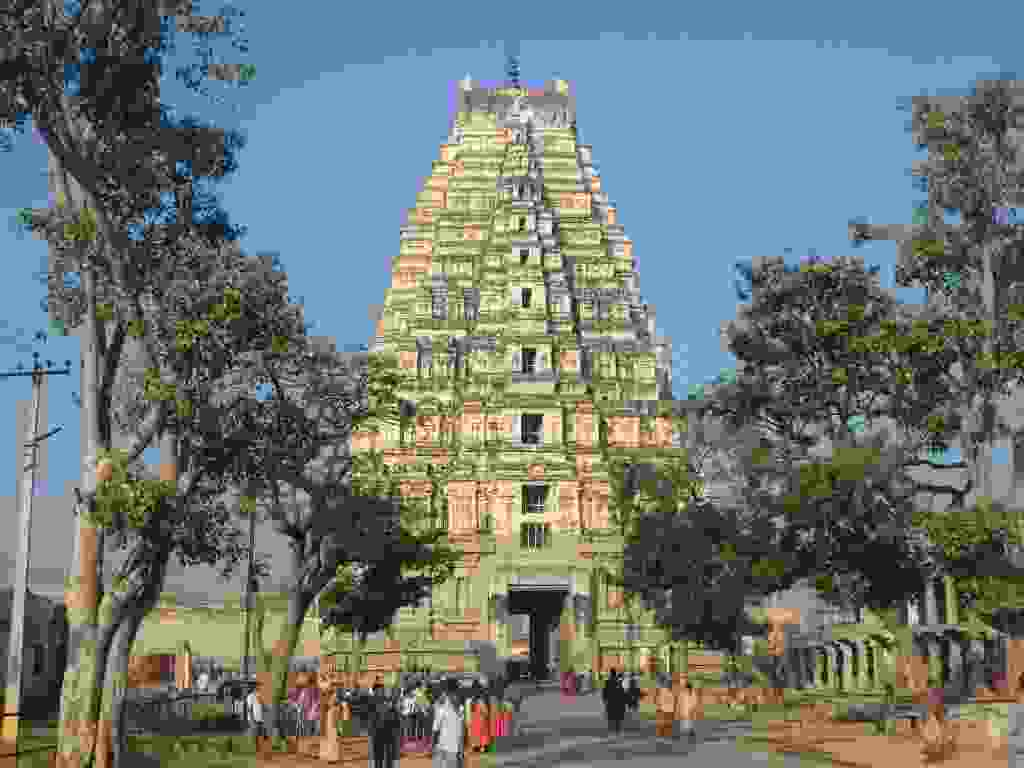
\includegraphics[width=\mywidth]{../wp-content/uploads/2015/12/PC181464-1024x768.jpg} } 
 \newline
 \newline
\centerline{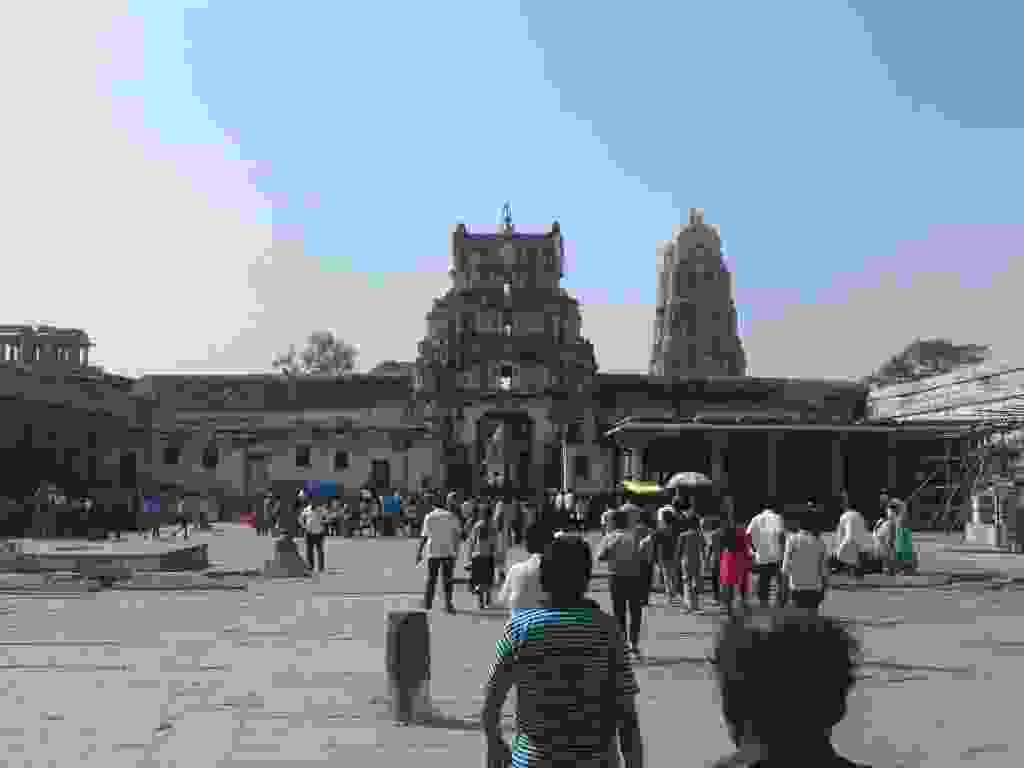
\includegraphics[width=\mywidth]{../wp-content/uploads/2015/12/PC181548-1024x768.jpg} } 
 \newline
 \newline
\centerline{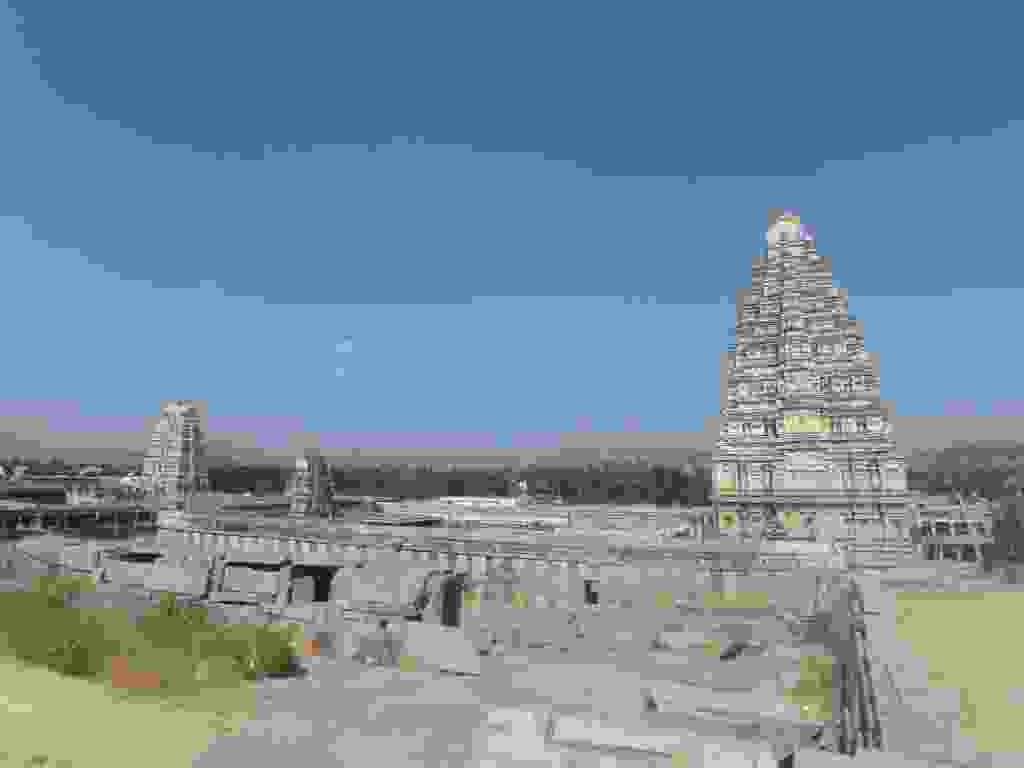
\includegraphics[width=\mywidth]{../wp-content/uploads/2015/12/PC181541-1024x768.jpg} } 
 \newline
 Les ruines de Vijayanâgara, ancienne capitale Hindoue, éparpillées tout autour de Hampi \newline
 \newline
\centerline{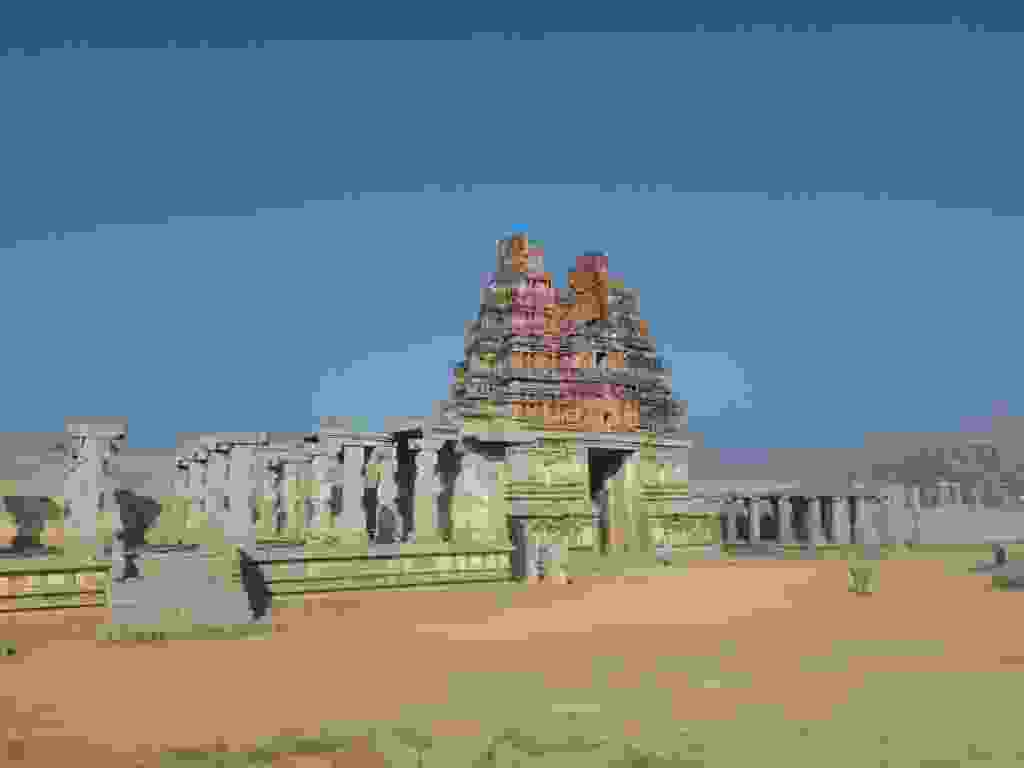
\includegraphics[width=\mywidth]{../wp-content/uploads/2015/12/PC181482-1024x768.jpg} } 
 \newline
 \newline
\centerline{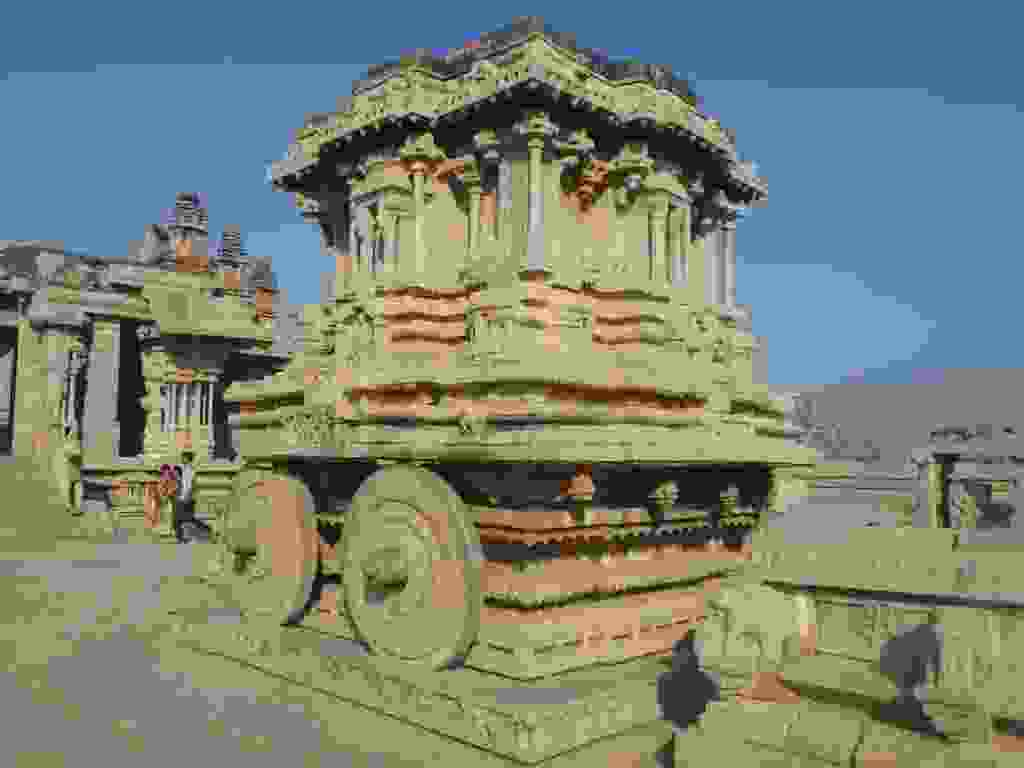
\includegraphics[width=\mywidth]{../wp-content/uploads/2015/12/PC181486-1024x768.jpg} } 
 \newline
 \newline
\centerline{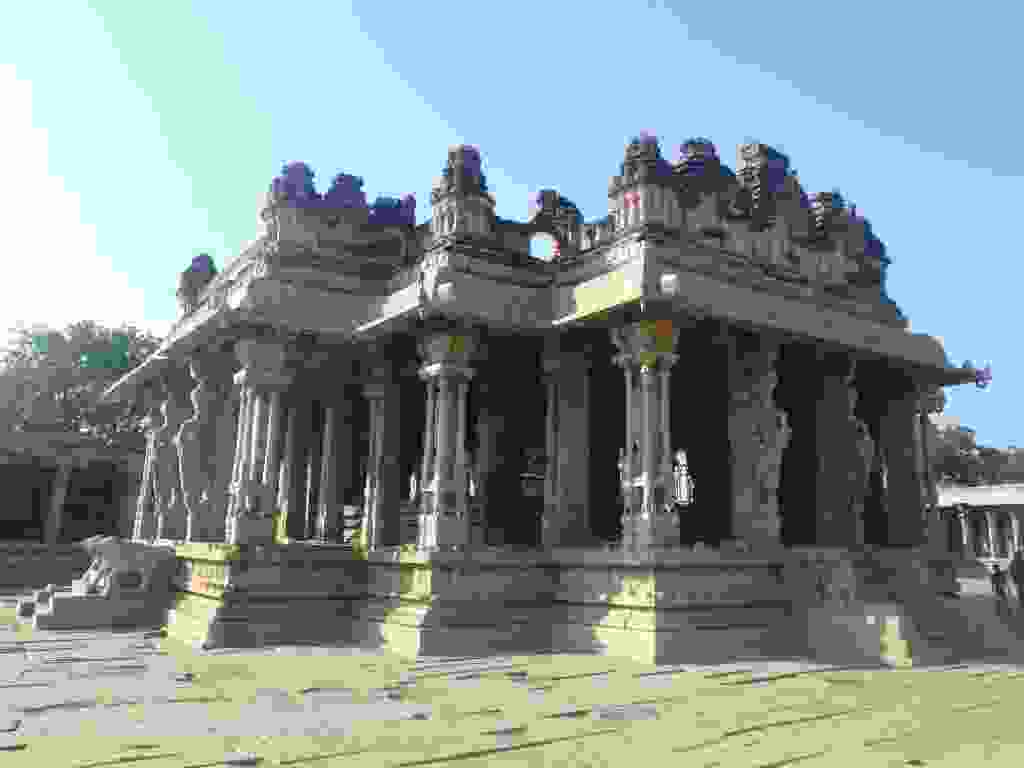
\includegraphics[width=\mywidth]{../wp-content/uploads/2015/12/PC181487-1024x768.jpg} } 
 \newline
 \newline
\centerline{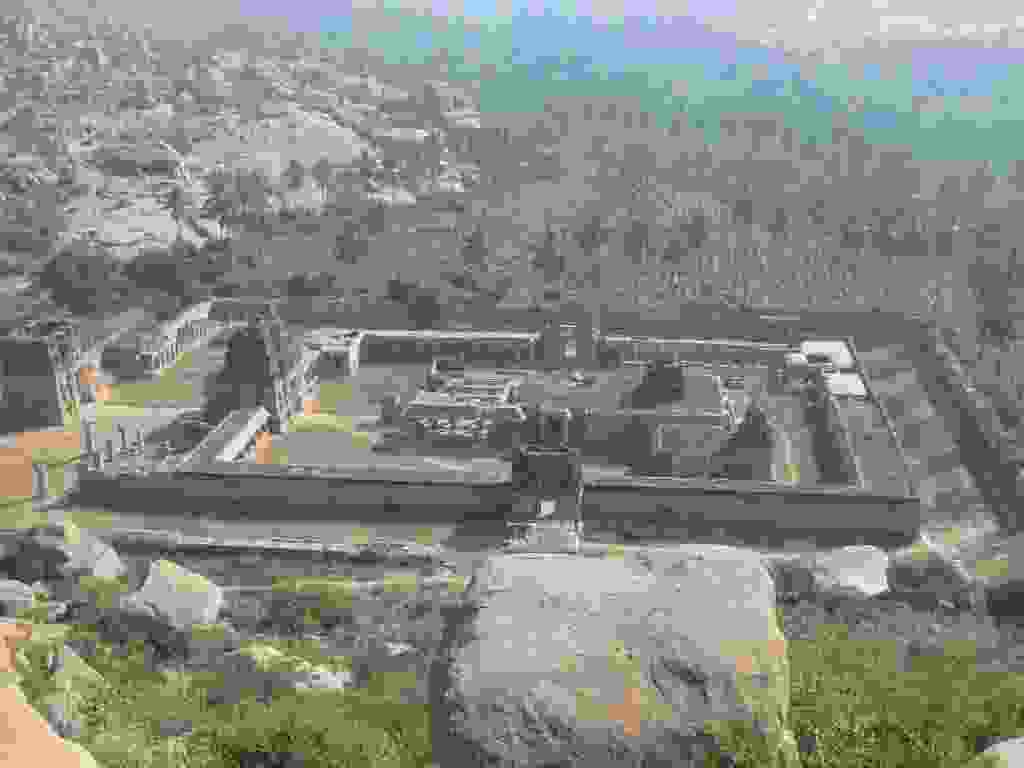
\includegraphics[width=\mywidth]{../wp-content/uploads/2015/12/PC181509-1024x768.jpg} } 
 \newline
 \newline
\centerline{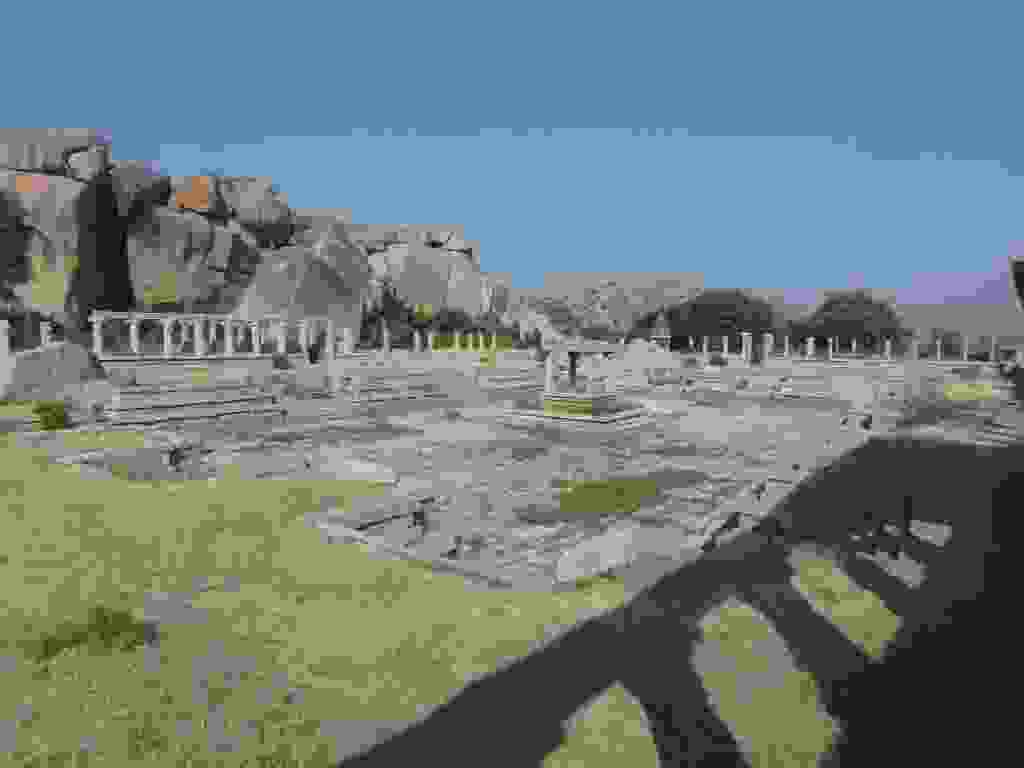
\includegraphics[width=\mywidth]{../wp-content/uploads/2015/12/PC181499-1024x768.jpg} } 
 \newline
 \newline
\centerline{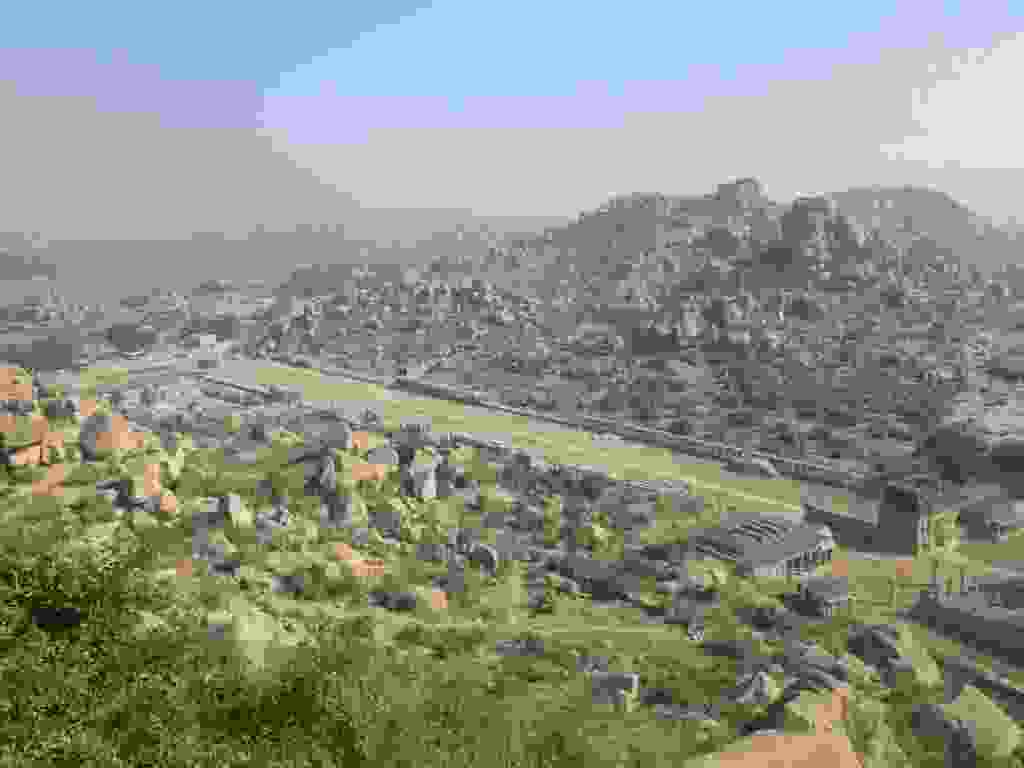
\includegraphics[width=\mywidth]{../wp-content/uploads/2015/12/PC181510-1024x768.jpg} } 
 \newline
 \newline
\centerline{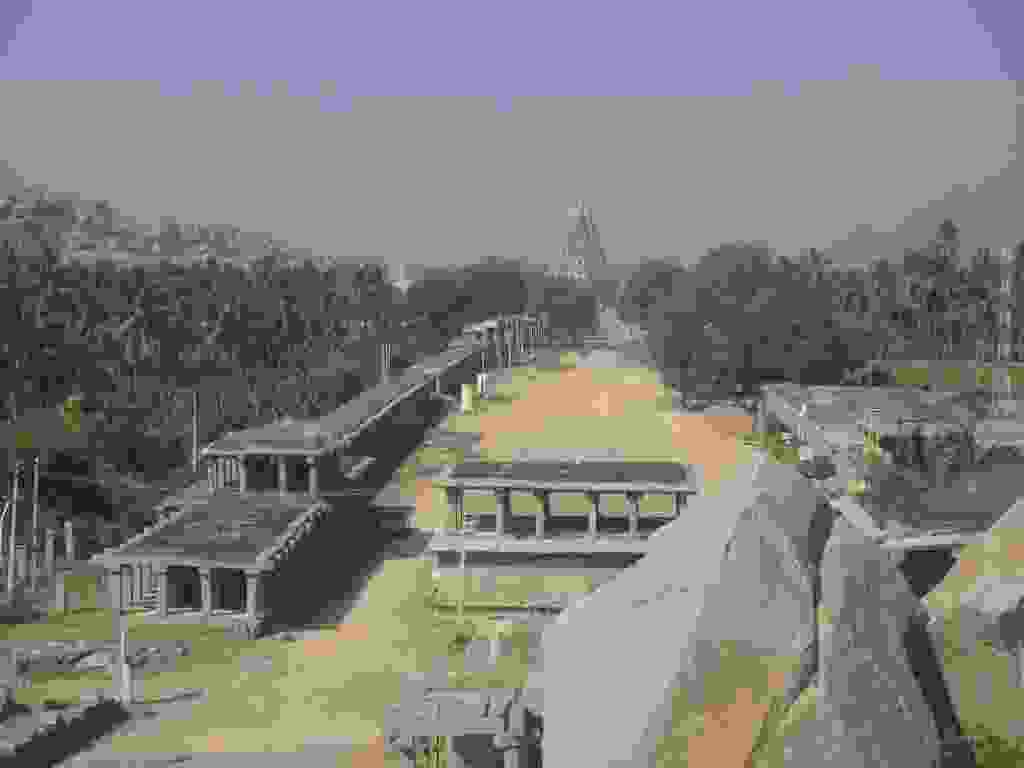
\includegraphics[width=\mywidth]{../wp-content/uploads/2015/12/PC181521-1024x768.jpg} } 
 \newline
 \newline
\centerline{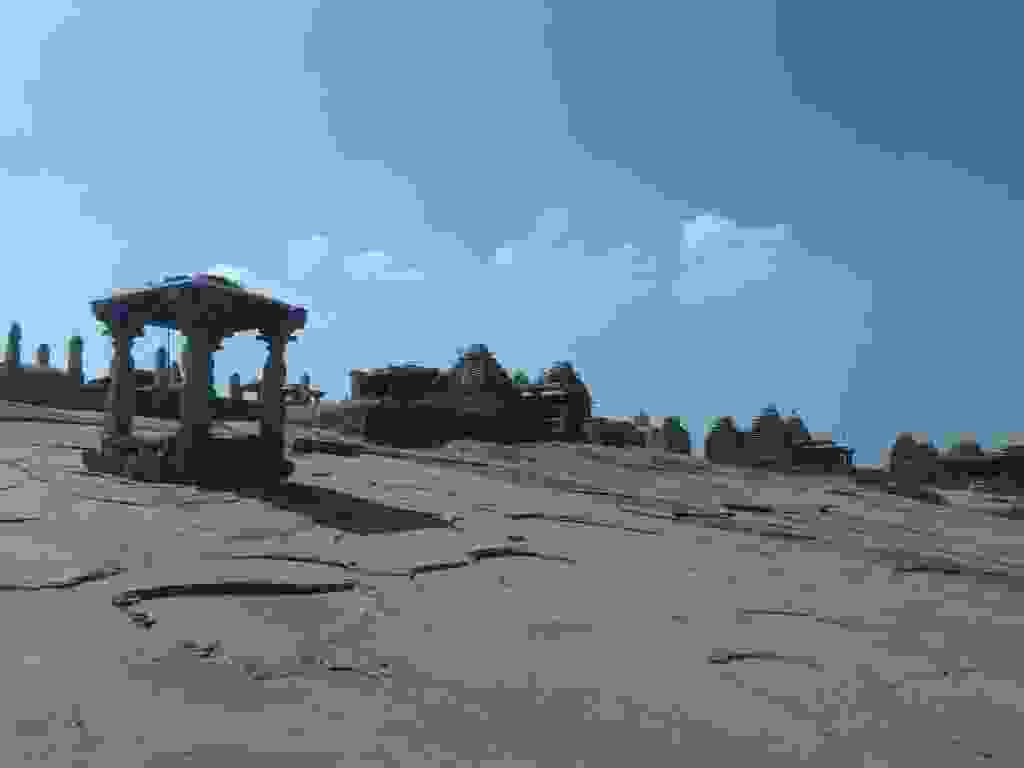
\includegraphics[width=\mywidth]{../wp-content/uploads/2015/12/PC181540-1024x768.jpg} } 
 \newline
 Lotus Mahal \newline
 \newline
\centerline{\includegraphics[width=\mywidth]{../wp-content/uploads/2015/12/PC181526-1024x768.jpg} } 
 \newline
 Etable pour éléphants \newline
 \newline
\centerline{\includegraphics[width=\mywidth]{../wp-content/uploads/2015/12/PC181529-1024x768.jpg} } 
 \newline
 Bains de la reine \newline
 \newline
\centerline{\includegraphics[width=\mywidth]{../wp-content/uploads/2015/12/PC181536-1024x768.jpg} } 
 \newline
 Dernière nuit de train pour rentrer à Bangalore, je récupère le vélo laissé chez Abhijit qui m'a hébergé \newline
 \newline
\centerline{\includegraphics[width=\mywidth]{../wp-content/uploads/2015/12/PC191554-1024x768.jpg} } 
 \newline
 Puis 30 km pour rejoindre l'aéroport et c'est la fin de 10 mois et demi de voyage ! \newline

\newpage
 
